
%% bare_jrnl_compsoc.tex
%% V1.4b
%% 2015/08/26
%% by Michael Shell
%% See:
%% http://www.michaelshell.org/
%% for current contact information.
%%
%% This is a skeleton file demonstrating the use of IEEEtran.cls
%% (requires IEEEtran.cls version 1.8b or later) with an IEEE
%% Computer Society journal paper.
%%
%% Support sites:
%% http://www.michaelshell.org/tex/ieeetran/
%% http://www.ctan.org/pkg/ieeetran
%% and
%% http://www.ieee.org/



% *** Authors should verify (and, if needed, correct) their LaTeX system  ***
% *** with the testflow diagnostic prior to trusting their LaTeX platform ***
% *** with production work. The IEEE's font choices and paper sizes can   ***
% *** trigger bugs that do not appear when using other class files.       ***                          ***
% The testflow support page is at:
% http://www.michaelshell.org/tex/testflow/


\documentclass[10pt,journal,compsoc]{IEEEtran}


%
% If IEEEtran.cls has not been installed into the LaTeX system files,
% manually specify the path to it like:
% \documentclass[10pt,journal,compsoc]{../sty/IEEEtran}





% Some very useful LaTeX packages include:
% (uncomment the ones you want to load)


% *** MISC UTILITY PACKAGES ***
%
%\usepackage{ifpdf}
% Heiko Oberdiek's ifpdf.sty is very useful if you need conditional
% compilation based on whether the output is pdf or dvi.
% usage:
% \ifpdf
%   % pdf code
% \else
%   % dvi code
% \fi
% The latest version of ifpdf.sty can be obtained from:
% http://www.ctan.org/pkg/ifpdf
% Also, note that IEEEtran.cls V1.7 and later provides a builtin
% \ifCLASSINFOpdf conditional that works the same way.
% When switching from latex to pdflatex and vice-versa, the compiler may
% have to be run twice to clear warning/error messages.

\usepackage{color}

\usepackage{graphicx}
\usepackage{caption}
\usepackage{subcaption}
\usepackage{wrapfig}
\usepackage{hyperref}

%for tables
\usepackage{booktabs}
\usepackage{makecell}

%for algorithm
\usepackage{algorithm}
\usepackage[noend]{algpseudocode}
\usepackage{varwidth}

\usepackage{etex}

%% editing comment
\newcommand{\cmt}[1]{{\footnotesize\textcolor{red}{#1}}}
\newcommand{\note}[1]{\cmt{Note: #1}}
\newcommand{\todo}[1]{\cmt{TO-DO: #1}}
\newcommand{\sergey}[1]{\cmt{Sergey: #1}}
\newcommand{\chelsea}[1]{\cmt{Chelsea: #1}}
\newcommand{\pieter}[1]{\cmt{Pieter: #1}}

%% ignore text
\long\def\ignorethis#1{}

%% abbreviations
\newcommand{\etal}{{et~al.}\ }
\newcommand{\eg}{e.g.\ }
\newcommand{\ie}{i.e.\ }
\newcommand{\nth}{\text{th}}
\newcommand{\pr}{^\prime}
\newcommand{\tr}{^\mathrm{T}}
\newcommand{\inv}{^{-1}}
\newcommand{\pinv}{^{\dagger}}
\newcommand{\real}{\mathbb{R}}
\newcommand{\gauss}{\mathcal{N}}
\newcommand{\norm}[1]{\left|#1\right|}
\newcommand{\trace}{\text{tr}}

%% defines autoref commands
\def\sectionautorefname{Section}
\let\subsectionautorefname\sectionautorefname
\let\subsubsectionautorefname\sectionautorefname
\providecommand\algorithmname{Algorithm}
\def\equationautorefname~#1\null{Equation~(#1)\null}
\def\appendixautorefname{Appendix}

%% reference shortcuts
\newcommand{\figtodo}[1]{\framebox[0.8\columnwidth]{\rule{0pt}{1in}#1}}
\newcommand{\figref}[1]{\autoref{#1}}
\renewcommand{\eqref}[1]{\autoref{#1}}
\newcommand{\secref}[1]{\autoref{#1}}

%% citation shortcuts
\newcommand{\atari}{acvpa-oglls-15}
\newcommand{\nyu}{vpbmse-mcl-16}

\newcommand{\model}{\mathcal{M}}
\newcommand{\action}{\mathbf{a}}
\newcommand{\state}{\mathbf{x}}
\newcommand{\image}{I_t}
\newcommand{\flow}{\hat{F}}
\newcommand{\pixel}{d} % the designated pixel
\newcommand{\pixelstate}{s} % the state of the desginated pixel
\newcommand{\goal}{g}




\usepackage{xcolor}  % for colored text
\providecommand\todo[1]{\textcolor{Red}{#1}}
\providecommand\edit[1]{\textcolor{blue}{#1}}



% *** CITATION PACKAGES ***
%
\ifCLASSOPTIONcompsoc
  % IEEE Computer Society needs nocompress option
  % requires cite.sty v4.0 or later (November 2003)
  \usepackage[nocompress]{cite}
\else
  % normal IEEE
  \usepackage{cite}
\fi
% cite.sty was written by Donald Arseneau
% V1.6 and later of IEEEtran pre-defines the format of the cite.sty package
% \cite{} output to follow that of the IEEE. Loading the cite package will
% result in citation numbers being automatically sorted and properly
% "compressed/ranged". e.g., [1], [9], [2], [7], [5], [6] without using
% cite.sty will become [1], [2], [5]--[7], [9] using cite.sty. cite.sty's
% \cite will automatically add leading space, if needed. Use cite.sty's
% noadjust option (cite.sty V3.8 and later) if you want to turn this off
% such as if a citation ever needs to be enclosed in parenthesis.
% cite.sty is already installed on most LaTeX systems. Be sure and use
% version 5.0 (2009-03-20) and later if using hyperref.sty.
% The latest version can be obtained at:
% http://www.ctan.org/pkg/cite
% The documentation is contained in the cite.sty file itself.
%
% Note that some packages require special options to format as the Computer
% Society requires. In particular, Computer Society  papers do not use
% compressed citation ranges as is done in typical IEEE papers
% (e.g., [1]-[4]). Instead, they list every citation separately in order
% (e.g., [1], [2], [3], [4]). To get the latter we need to load the cite
% package with the nocompress option which is supported by cite.sty v4.0
% and later. Note also the use of a CLASSOPTION conditional provided by
% IEEEtran.cls V1.7 and later.





% *** GRAPHICS RELATED PACKAGES ***
%
\ifCLASSINFOpdf
  % \usepackage[pdftex]{graphicx}
  % declare the path(s) where your graphic files are
  % \graphicspath{{../pdf/}{../jpeg/}}
  % and their extensions so you won't have to specify these with
  % every instance of \includegraphics
  % \DeclareGraphicsExtensions{.pdf,.jpeg,.png}
\else
  % or other class option (dvipsone, dvipdf, if not using dvips). graphicx
  % will default to the driver specified in the system graphics.cfg if no
  % driver is specified.
  % \usepackage[dvips]{graphicx}
  % declare the path(s) where your graphic files are
  % \graphicspath{{../eps/}}
  % and their extensions so you won't have to specify these with
  % every instance of \includegraphics
  % \DeclareGraphicsExtensions{.eps}
\fi
% graphicx was written by David Carlisle and Sebastian Rahtz. It is
% required if you want graphics, photos, etc. graphicx.sty is already
% installed on most LaTeX systems. The latest version and documentation
% can be obtained at: 
% http://www.ctan.org/pkg/graphicx
% Another good source of documentation is "Using Imported Graphics in
% LaTeX2e" by Keith Reckdahl which can be found at:
% http://www.ctan.org/pkg/epslatex
%
% latex, and pdflatex in dvi mode, support graphics in encapsulated
% postscript (.eps) format. pdflatex in pdf mode supports graphics
% in .pdf, .jpeg, .png and .mps (metapost) formats. Users should ensure
% that all non-photo figures use a vector format (.eps, .pdf, .mps) and
% not a bitmapped formats (.jpeg, .png). The IEEE frowns on bitmapped formats
% which can result in "jaggedy"/blurry rendering of lines and letters as
% well as large increases in file sizes.
%
% You can find documentation about the pdfTeX application at:
% http://www.tug.org/applications/pdftex






% *** MATH PACKAGES ***
%
%\usepackage{amsmath}
% A popular package from the American Mathematical Society that provides
% many useful and powerful commands for dealing with mathematics.
%
% Note that the amsmath package sets \interdisplaylinepenalty to 10000
% thus preventing page breaks from occurring within multiline equations. Use:
%\interdisplaylinepenalty=2500
% after loading amsmath to restore such page breaks as IEEEtran.cls normally
% does. amsmath.sty is already installed on most LaTeX systems. The latest
% version and documentation can be obtained at:
% http://www.ctan.org/pkg/amsmath

\usepackage{amsmath}
\usepackage{amsfonts}
\usepackage{mathtools}



% *** SPECIALIZED LIST PACKAGES ***
%
%\usepackage{algorithmic}
% algorithmic.sty was written by Peter Williams and Rogerio Brito.
% This package provides an algorithmic environment fo describing algorithms.
% You can use the algorithmic environment in-text or within a figure
% environment to provide for a floating algorithm. Do NOT use the algorithm
% floating environment provided by algorithm.sty (by the same authors) or
% algorithm2e.sty (by Christophe Fiorio) as the IEEE does not use dedicated
% algorithm float types and packages that provide these will not provide
% correct IEEE style captions. The latest version and documentation of
% algorithmic.sty can be obtained at:
% http://www.ctan.org/pkg/algorithms
% Also of interest may be the (relatively newer and more customizable)
% algorithmicx.sty package by Szasz Janos:
% http://www.ctan.org/pkg/algorithmicx




% *** ALIGNMENT PACKAGES ***
%
%\usepackage{array}
% Frank Mittelbach's and David Carlisle's array.sty patches and improves
% the standard LaTeX2e array and tabular environments to provide better
% appearance and additional user controls. As the default LaTeX2e table
% generation code is lacking to the point of almost being broken with
% respect to the quality of the end results, all users are strongly
% advised to use an enhanced (at the very least that provided by array.sty)
% set of table tools. array.sty is already installed on most systems. The
% latest version and documentation can be obtained at:
% http://www.ctan.org/pkg/array


% IEEEtran contains the IEEEeqnarray family of commands that can be used to
% generate multiline equations as well as matrices, tables, etc., of high
% quality.

%for tables
\usepackage{makecell}




% *** SUBFIGURE PACKAGES ***
%\ifCLASSOPTIONcompsoc
%  \usepackage[caption=false,font=footnotesize,labelfont=sf,textfont=sf]{subfig}
%\else
%  \usepackage[caption=false,font=footnotesize]{subfig}
%\fi
% subfig.sty, written by Steven Douglas Cochran, is the modern replacement
% for subfigure.sty, the latter of which is no longer maintained and is
% incompatible with some LaTeX packages including fixltx2e. However,
% subfig.sty requires and automatically loads Axel Sommerfeldt's caption.sty
% which will override IEEEtran.cls' handling of captions and this will result
% in non-IEEE style figure/table captions. To prevent this problem, be sure
% and invoke subfig.sty's "caption=false" package option (available since
% subfig.sty version 1.3, 2005/06/28) as this is will preserve IEEEtran.cls
% handling of captions.
% Note that the Computer Society format requires a sans serif font rather
% than the serif font used in traditional IEEE formatting and thus the need
% to invoke different subfig.sty package options depending on whether
% compsoc mode has been enabled.
%
% The latest version and documentation of subfig.sty can be obtained at:
% http://www.ctan.org/pkg/subfig




% *** FLOAT PACKAGES ***
%
%\usepackage{fixltx2e}
% fixltx2e, the successor to the earlier fix2col.sty, was written by
% Frank Mittelbach and David Carlisle. This package corrects a few problems
% in the LaTeX2e kernel, the most notable of which is that in current
% LaTeX2e releases, the ordering of single and double column floats is not
% guaranteed to be preserved. Thus, an unpatched LaTeX2e can allow a
% single column figure to be placed prior to an earlier double column
% figure.
% Be aware that LaTeX2e kernels dated 2015 and later have fixltx2e.sty's
% corrections already built into the system in which case a warning will
% be issued if an attempt is made to load fixltx2e.sty as it is no longer
% needed.
% The latest version and documentation can be found at:
% http://www.ctan.org/pkg/fixltx2e


%\usepackage{stfloats}
% stfloats.sty was written by Sigitas Tolusis. This package gives LaTeX2e
% the ability to do double column floats at the bottom of the page as well
% as the top. (e.g., "\begin{figure*}[!b]" is not normally possible in
% LaTeX2e). It also provides a command:
%\fnbelowfloat
% to enable the placement of footnotes below bottom floats (the standard
% LaTeX2e kernel puts them above bottom floats). This is an invasive package
% which rewrites many portions of the LaTeX2e float routines. It may not work
% with other packages that modify the LaTeX2e float routines. The latest
% version and documentation can be obtained at:
% http://www.ctan.org/pkg/stfloats
% Do not use the stfloats baselinefloat ability as the IEEE does not allow
% \baselineskip to stretch. Authors submitting work to the IEEE should note
% that the IEEE rarely uses double column equations and that authors should try
% to avoid such use. Do not be tempted to use the cuted.sty or midfloat.sty
% packages (also by Sigitas Tolusis) as the IEEE does not format its papers in
% such ways.
% Do not attempt to use stfloats with fixltx2e as they are incompatible.
% Instead, use Morten Hogholm'a dblfloatfix which combines the features
% of both fixltx2e and stfloats:
%
\usepackage{dblfloatfix}
% The latest version can be found at:
% http://www.ctan.org/pkg/dblfloatfix



%\ifCLASSOPTIONcaptionsoff
%  \usepackage[nomarkers]{endfloat}
% \let\MYoriglatexcaption\caption
% \renewcommand{\caption}[2][\relax]{\MYoriglatexcaption[#2]{#2}}
%\fi
% endfloat.sty was written by James Darrell McCauley, Jeff Goldberg and 
% Axel Sommerfeldt. This package may be useful when used in conjunction with 
% IEEEtran.cls'  captionsoff option. Some IEEE journals/societies require that
% submissions have lists of figures/tables at the end of the paper and that
% figures/tables without any captions are placed on a page by themselves at
% the end of the document. If needed, the draftcls IEEEtran class option or
% \CLASSINPUTbaselinestretch interface can be used to increase the line
% spacing as well. Be sure and use the nomarkers option of endfloat to
% prevent endfloat from "marking" where the figures would have been placed
% in the text. The two hack lines of code above are a slight modification of
% that suggested by in the endfloat docs (section 8.4.1) to ensure that
% the full captions always appear in the list of figures/tables - even if
% the user used the short optional argument of \caption[]{}.
% IEEE papers do not typically make use of \caption[]'s optional argument,
% so this should not be an issue. A similar trick can be used to disable
% captions of packages such as subfig.sty that lack options to turn off
% the subcaptions:
% For subfig.sty:
% \let\MYorigsubfloat\subfloat
% \renewcommand{\subfloat}[2][\relax]{\MYorigsubfloat[]{#2}}
% However, the above trick will not work if both optional arguments of
% the \subfloat command are used. Furthermore, there needs to be a
% description of each subfigure *somewhere* and endfloat does not add
% subfigure captions to its list of figures. Thus, the best approach is to
% avoid the use of subfigure captions (many IEEE journals avoid them anyway)
% and instead reference/explain all the subfigures within the main caption.
% The latest version of endfloat.sty and its documentation can obtained at:
% http://www.ctan.org/pkg/endfloat
%
% The IEEEtran \ifCLASSOPTIONcaptionsoff conditional can also be used
% later in the document, say, to conditionally put the References on a 
% page by themselves.




% *** PDF, URL AND HYPERLINK PACKAGES ***
%
%\usepackage{url}
% url.sty was written by Donald Arseneau. It provides better support for
% handling and breaking URLs. url.sty is already installed on most LaTeX
% systems. The latest version and documentation can be obtained at:
% http://www.ctan.org/pkg/url
% Basically, \url{my_url_here}.





% *** Do not adjust lengths that control margins, column widths, etc. ***
% *** Do not use packages that alter fonts (such as pslatex).         ***
% There should be no need to do such things with IEEEtran.cls V1.6 and later.
% (Unless specifically asked to do so by the journal or conference you plan
% to submit to, of course. )


% correct bad hyphenation here
\hyphenation{op-tical net-works semi-conduc-tor}


\begin{document}
%
% paper title
% Titles are generally capitalized except for words such as a, an, and, as,
% at, but, by, for, in, nor, of, on, or, the, to and up, which are usually
% not capitalized unless they are the first or last word of the title.
% Linebreaks \\ can be used within to get better formatting as desired.
% Do not put math or special symbols in the title.
%\title{Deep Reinforcement Learning with Observation Models}
\title{Visual Foresight: Model-Based Deep Reinforcement Learning for Vision-Based Robotic Control}
%14: I think the current title is a bit too aggressive -- kind of makes it seem like all the other RL is not "real." We should make sure to hit a few key words: we need to make sure the title communicates that this is based on images, that there is robotic manipulation going on, and that it is based on prediction or something like that. We should also pick a name for the method. I don't particularly like "Visual MPC" (it sounds a bit antiquated, like visual servoing), but if we go with that, we can call it
%Visual MPC: Model-Based Deep Reinforcement Learning for Vision-Based Robotic Control
% we can also go with "foresight" and call it
%Visual Foresight: Deep Reinforcement Learning via Prediction for Vision-Based Robotic Control
%% Real-World Deep Reinforcement Learning with Sensory Prediction Models
%% TITLE IDEAS HERE (separate from method names)
% Learning Observation Models for Real-World Planning and Control
% Deep Reinforcement Learning from Images with Observation Models
% Observation Models for Scalable, Real-World Reinforcement Learning
% Observation Models for Scalable Deep Reinforcement Learning
%
% Robotic Manipluation using Video Prediction Models
% Deep Model-Based Reinforcement Learning for Real-World Visual Control
% Deep Visual Predictive Models for Control
% Predictive Models for Visual Planning
% Deep Predictive Models for Visual Planning
% Learning Visual Foresight for Robotic Manipulation
% Observation Models for Self-Supervised Planning and Control
% Learning Observation Models for Real-World Planning and Control
% Learning Observation Models for Planning and Control
% Observation Models for Real-World Reinforcement Learning
%
% Sensory Prediction Models for Real-World Reinforcement Learning
% Sensory Prediction Models for Real-World Deep Reinforcement Learning

\author{Frederik Ebert*, Chelsea Finn*, Annie Xie, Sudeep Dasari, Alex Lee, Sergey Levine
%Frederik Ebert, Chelsea Finn, Alex Lee, Annie Xie, Sudeep Dasari, Sergey Levine
        
\IEEEcompsocitemizethanks{
\IEEEcompsocthanksitem  The first two authors contributed equally.}% <-this % stops an unwanted space
\thanks{Manuscript received 11/22/2018}}

% note the % following the last \IEEEmembership and also \thanks - 
% these prevent an unwanted space from occurring between the last author name
% and the end of the author line. i.e., if you had this:
% 
% \author{....lastname \thanks{...} \thanks{...} }
%                     ^------------^------------^----Do not want these spaces!
%
% a space would be appended to the last name and could cause every name on that
% line to be shifted left slightly. This is one of those "LaTeX things". For
% instance, "\textbf{A} \textbf{B}" will typeset as "A B" not "AB". To get
% "AB" then you have to do: "\textbf{A}\textbf{B}"
% \thanks is no different in this regard, so shield the last } of each \thanks
% that ends a line with a % and do not let a space in before the next \thanks.
% Spaces after \IEEEmembership other than the last one are OK (and needed) as
% you are supposed to have spaces between the names. For what it is worth,
% this is a minor point as most people would not even notice if the said evil
% space somehow managed to creep in.



% The paper headers
\markboth{Journal of \LaTeX\ Class Files,~Vol.~14, No.~8, August~2015}%
{Shell \MakeLowercase{\textit{et al.}}: Bare Demo of IEEEtran.cls for Computer Society Journals}
% The only time the second header will appear is for the odd numbered pages
% after the title page when using the twoside option.
% 
% *** Note that you probably will NOT want to include the author's ***
% *** name in the headers of peer review papers.                   ***
% You can use \ifCLASSOPTIONpeerreview for conditional compilation here if
% you desire.



% The publisher's ID mark at the bottom of the page is less important with
% Computer Society journal papers as those publications place the marks
% outside of the main text columns and, therefore, unlike regular IEEE
% journals, the available text space is not reduced by their presence.
% If you want to put a publisher's ID mark on the page you can do it like
% this:
%\IEEEpubid{0000--0000/00\$00.00~\copyright~2015 IEEE}
% or like this to get the Computer Society new two part style.
%\IEEEpubid{\makebox[\columnwidth]{\hfill 0000--0000/00/\$00.00~\copyright~2015 IEEE}%
%\hspace{\columnsep}\makebox[\columnwidth]{Published by the IEEE Computer Society\hfill}}
% Remember, if you use this you must call \IEEEpubidadjcol in the second
% column for its text to clear the IEEEpubid mark (Computer Society jorunal
% papers don't need this extra clearance.)



% use for special paper notices
%\IEEEspecialpapernotice{(Invited Paper)}

% for Computer Society papers, we must declare the abstract and index terms
% PRIOR to the title within the \IEEEtitleabstractindextext IEEEtran
% command as these need to go into the title area created by \maketitle.
% As a general rule, do not put math, special symbols or citations
% in the abstract or keywords.
\IEEEtitleabstractindextext{%
\begin{abstract}
Deep reinforcement learning (RL) algorithms can learn complex robotic skills from raw sensory inputs, but have yet to achieve the kind of broad generalization and applicability demonstrated by deep learning methods in supervised domains. We present a deep RL method that is practical for real-world robotics tasks, such as robotic manipulation, and generalizes effectively to never-before-seen tasks and objects. In these settings, ground truth reward signals are typically unavailable, and we therefore propose a self-supervised model-based approach, where a predictive model learns to directly predict the future from raw sensory readings, such as camera images. At test time, we explore three distinct goal specification methods: designated pixels, where a user specifies desired object manipulation tasks by selecting particular pixels in an image and corresponding goal positions, goal images, where the desired goal state is specified with an image, and image classifiers, which define spaces of goal states. Our deep predictive models are trained using data collected autonomously and continuously by a robot interacting with hundreds of objects, without human supervision. We demonstrate that visual MPC can generalize to never-before-seen objects---both rigid and deformable---and solve a range of user-defined object manipulation tasks using the same model.
\end{abstract}

% Note that keywords are not normally used for peerreview papers.
\begin{IEEEkeywords}
Deep Reinforcement Learning, Video Prediction, Robotic Manipulation, Model Predictive Control
\end{IEEEkeywords}}

% make the title area
\maketitle

% To allow for easy dual compilation without having to reenter the
% abstract/keywords data, the \IEEEtitleabstractindextext text will
% not be used in maketitle, but will appear (i.e., to be "transported")
% here as \IEEEdisplaynontitleabstractindextext when the compsoc 
% or transmag modes are not selected <OR> if conference mode is selected 
% - because all conference papers position the abstract like regular
% papers do.
\IEEEdisplaynontitleabstractindextext
% \IEEEdisplaynontitleabstractindextext has no effect when using
% compsoc or transmag under a non-conference mode.


\IEEEpeerreviewmaketitle

\IEEEraisesectionheading{\section{Introduction}\label{sec:introduction}}

current approaches for general-purpose robotic manipulation can be loosely categorized into two schools: The first where algorithms are designed, trained or tuned in simulation and then deployed in the real world. While simulation has the advantage of being cheaper and running orders of magnitudes faster it also often comes at a price: Many real-world phenomena such as complex friction, soft-objects, liquids or even other agents such as humans often cannot be modeled with sufficient fidelity. Therefore the resulting policies often do not transfer very well from simulation the real world.

A completely different approach is to avoid simulation and manual feature engineering and instead learn models and policies through interacting with the real world. This typically requires human resets and complex hand-engineered reward functions. For example \cite{DBLP:journals/corr/GuHLL16} presents a method for learning door opening using robot manipulators in the real world while humans are required to perform hundreds of resets in addition to sensors measuring the success of the door opening task.

Here we present a family of methods (extending our work in \cite{foresight}, \cite{sna}, \todo{cite robustness from retry, SAVP, classifier VMPC}) that enable robots to learn complex manipulation skills from interacting with their environment requiring \emph{very little or no human supervision at all}. We show that the need for human supervision can be removed by training an action-conditioned video-prediction model from data that is collected completely autonomously by the robot interacting with its environment. This work demonstrates that by training the model on the task of predicting what it will see next (for a given sequence of motor commands) it learns models of environment dynamics that can be used effectively for robotic control.

In the proposed approach neither models of the robot nor the environment dynamics need to be provided ahead of time, since the action-conditioned prediction model is learned purely on autonomously collected data.

For video-prediction-based control a specific type of model -- transformation-based video-prediction -- has proven to be particularly effective. One of the reasons is that the transformations can be used to obtain predictions of \emph{where} certain pixels in the image are moving. However due to occlusion (of objects by the arm) severe limitations for planning performance can arise when planning costs are computed from transformation-based predictions. We propose type of video-prediction model that uses temporal skip connections to recover parts of the images that are occluded during the predictions and demonstrates that this yields significant improvements for manipulation planning.\

\todo{mention stochastic video prediction in case improvements are observed}

To achieve complex long-term behaviour the ability to correct for mistakes due to uncertainty and accumulating erros in the models predictions is a key requirement. If the agent can always evaluate the goal (along its predictions), it can continuously retry, so that even flawed predictions allow for an eventual successful execution. To this end we propose a cost function for video-prediction based planning based on image registration, which we demonstrate can itself be learned on the same dataset as the one used to train the predictive model. This closed-loop visual control allows the robot to be persistent, correcting for mistakes caused by inevitable model inaccuracies allowing it to retry indefinitely until it succeeds.

\todo{motivate one-shot classifier based control}

The technical contribution of this work is four-fold. First, we present a video-prediction-based method for robotic control that enables learning complex manipulation skills \emph{purely from autonomously collected data}. Second we show that the video-prediction model's capability to \emph{accurately maintain object permanence through occlusions} can be enhanced by incorporating temporal skip connections. Third we propose a method for allowing \emph{closed loop control} equipping the agent with the ability to retry the task indefinitely until it succeeds which contributes significantly to the method's robustness. Fourth a cost function based on a few-shot classifier-based is presented which allows the agent to successfully \emph{execute tasks defined by a single demonstration}.

Our evaluation demonstrates that these components can be combined to enable a learned video prediction model to perform a range of real-world pushing tasks. Our experiments include manipulation of previously unseen objects, handling multiple objects, pushing objects around obstructions, and moving the arm around and over other obstacle-objects, recovering from large perturbations, grasping objects and maneuvering them to a user-specified point in 3D-space representing a significant advance in the range and complexity of skills that can be acquired through entirely self-supervised learning.

 






% Motivate self-supervised learning
% discuss relationship with reinforcement learning

\section{Related Work}\label{sec:rel_work}

%%SL.10.15: changed subsection to \paragraph -- don't have hanging subsections without any text between \section and \subsection
\textbf{Learning from rewards.}
Reinforcement learning typically assumes access to an external reward signal, effectively \emph{reinforcing} good behavior \cite{lillicrap2015continuous, sutton1998reinforcement}. Our approach learns a \emph{goal-agnostic} model without any external rewards, and then uses this model to plan to achieve user-specified goals at test-time.
A wide range of tasks can be solved by defining appropriate \emph{internal} cost functions. These internal costs are computed based on rollouts of the sensory prediction model, as detailed in section \ref{sec:cost}.
%%SL.10.15: This is not the place to discuss MPC, because MPC does not learn from rewards. However, the above paragraph should have some citations -- what's the point of having a related work paragraph that doesn't actually summarize any related work?
%Thus our method is reminiscent of model-predictive control (MPC), but instead of an analytical, hand-designed model, we employ a deep sensory prediction model.

%%SL.10.15: We need a paragraph about model-based RL somewhere here. Maybe something like this:
\noindent \textbf{Model-based reinforcement learning.} Learning a model to predict the future, and then using this model to act, falls under the general umbrella of model-based reinforcement learning. Model-based algorithms are generally known to be more efficient than model-free methods~\cite{chua2018deep, deisenroth2013survey}, and have been used with both low-dimensional~\cite{deisenroth2011pilco} and high-dimensional~\cite{nagabandi2017neural} model classes. However, model-based RL methods that directly operate on raw image frames have not been studied as extensively. Several algorithms have been proposed for simple, synthetic images~\cite{watter2015embed} and video game environments~\cite{ha2018world}, but have not been evaluated on generalization or in the real world, and recent work has also studied model-based RL for individual robotic skills~\cite{zhang2018solar}. In contrast to these works, we place special emphasis on \emph{generalization}, studying how predictive models can enable a real robot to manipulate previously unseen objects.

\noindent \textbf{Self-supervised robotic learning.}
A number of recent works have studied self-supervised robotic learning, where large-scale unattended data collection is used to learn individual skills such as grasping~\cite{mottaghi2016happens, lerrel,google_handeye} or obstacle avoidance~\cite{greg_kahn_uncertainty,crashing}. 
%%CF.11.04: Add Vladlen's "learning to act by predicting the future" paper to the above sentence, which also predicts future "events".
 reviewers. \todo{Also cite Roberto's paper probably.}
In contrast to these methods, our approach learns predictive models that can be used to perform a variety of manipulation skills, and does not require a success measure, event indicator, or reward function during data collection. 

%%CF.11.04: Inverse models should go in the model-based RL section, I think.
Prior work has also used ``inverse models,'' which learn to predict actions that lead from one state to another state specified by sensory inputs, to learn skills such as object pushing~\cite{agrawal2016learning} and rope tying~\cite{nair2017combining}.
Pinto et al. \cite{pinto2016curious} perform self-supervised learning in a multi-task setting combing learning an inverse model for pushing, a grasp success metric and pose-invariant image embeddings.
%%SL.10.15: This should cite Ashvin's 2017 ICRA paper on rope manipulation.
However, such methods struggle when applied to more extended or continuous tasks, where their inability to support forward planning and tendency to pick up on extraneous distractors (e.g., predicting the action just from observing the arm) present severe challenges. We observe a substantial improvement in the length and complexity of manipulations that can be performed with our method.
%%SL.10.15: is there any evidence (at least in sim?) we can show to back up this last assertion?

%Thanard's model:
Kurutach et al. use a InfoGAN model \cite{kurutach2018learning} to learn a latent-space describing the environment states in which planning can be performed. The model can be used to obtain a sequence of waypoints in the latent space between the current state and goal-state. The method currently relies on an inverse model to reach the states proposed by the InfoGAN model. So far experiments have been limited to rope rearrangement tasks.
%%SL.10.15: I don't think that paper has any rope rearrangement, just some results showing predictions? But maybe more to the point, we should probably just have a broader discussion of video prediction models, and put this citation somewhere in the middle of that. It seems weird to single it out among the other predictive models papers. I would just suggest deleting this paragraph and working the citation somewhere into the next paragraph.
%%CF.11.04: don't forget to address the above.

\noindent \textbf{Sensory prediction models.}
We propose to leverage sensory prediction models, such as video-prediction models, to enable large-scale self-supervised learning of robotic skills. Prior work on video prediction has studied synthetic video game images~\cite{atarioh,recurrentsimulators} and robotic manipulation~\cite{bootsetal,finn_nips,video_pixel_networks}. Video prediction without actions has been studied for unstructured videos~\cite{beyond_mse,convlstm,vondrick} and driving~\cite{prednet,dynamic_filter_networks}. Several works have sought to use more complex distributions for future images, for example by using autoregressive models~\cite{video_pixel_networks,scott_reed}. While this often produces sharp predictions, the resulting models are extremely demanding computationally which would be impractical for real-world robotic control. In this work, we extend video prediction methods that are based on predicting a transformation from the previous image~\cite{finn_nips,dynamic_filter_networks}. Prior work has also sought to predict motion directly in 3D, using 3D point clouds obtained from a depth camera~\cite{se3}, requiring point-to-point correspondences over time, which makes it hard to apply to previously unseen objects. Our predictive model is effective for a wide range of real-world object manipulations and does not require 3D depth sensing or point-to-point correspondences between frames. Crucially, we demonstrate that our models enable real-world robotic control, making it possible to perform a variety of user-specified manipulation tasks.
%%CF.11.04: maybe also state that advances in video prediction are complementary to our approach.

% discuss related work on video-prediction
% on model-predictive control (e.g. Anusha's work)
% visual servoing
% environment modeling e.g. interaction networks

\section{Overview}\label{sec:prelim}
\label{sec:vmpc}
%%SL.10.15: change title to Overview?

%%SL.10.15: This is the wrong level of abstraction for this section. This section should provide a high-level overview of the structure of the method: data collection (how is that done?), model training, some considerations about the model (what is input and what is output?) and a brief summary of the test-time control method, not at the level of designated pixels yet, but maybe with a short summary of different ways to specify costs and some details about planning. I recommend starting with a high level motivation sentence or two, and then having \textbf{} paragraph headings for "Training data collection" "Model training" and "Test-time control", then briefly summarize what the following sections will be about, something like "In the next section, we will discuss the architectures and training procedures for our predictive models, followed by a discussion of planning objectives in Section~\ref{sec:something}, planning in Section~\ref{sec:something}, and system design considerations in Section~\ref{sec:something}." Here is an example for how you can open with the high level motivation: 
In this section, we summarize our visual model-predictive control (MPC) approach, which consists of a model-based reinforcement learning approach to end-to-end learning of robotic manipulation skills. Our method, outlined in figure \ref{fig:overview}, consists of three phases: unsupervised data collection, predictive model training, and planning-based control via the model at test-time.

\textbf{Unsupervised data collection}: At \emph{training time}, data is collected autonomously by applying random actions sampled from a pre-specified distribution. It is important that this distribution allows the robot to visit parts of the state space that are relevant for solving the intended tasks. Therefore we design a custom sampling distribution to direct data collection to the desired parts of the state space, as further detailed in Sections \ref{sec:system} and \ref{subsec:cloth_folding_data}.

\textbf{Model training}: A video-prediction model is trained on the collected data offline. The video-prediction model takes as input an image of the current time-step and a sequence of actions, and generates the corresponding sequence of future frames. The video-prediction model is detailed in Section \ref{sec:model}.

\textbf{Test-time control}: At \emph{test time} we use a sampling-based, gradient free optimization procedure, similar to ``shooting methods``, to find the sequence of actions that minimizes a cost function. Further details, including the motivation for this type of optimizer, can be found in Section \ref{sec:optimizer}. 

Depending on how the goal is specified, we use one of the following three cost functions: When the goal is provided by clicking on an object and a desired goal-position, a \emph{pixel-distance cost-function}, detailed in Section \ref{subsec:pixel_dist_cost}, is used that evaluates how far the designated pixel is from the goal pixels. We can specify the goal more precisely by providing a goal-image in addition to the pixel positions and make use of \emph{image-to-image registration} to compute a cost function, this is explained in Section \ref{subsec:reg_cost}. Finally we show that more abstract tasks can be solved by providing one or several demonstrations and employing a classifier-based cost function as detailed in Section \ref{subsec:class_cost}. The strengths and weaknesses of different costs functions and trade-offs between them are discussed in Section \ref{subsec:cost_discuission}. 

The model is used to plan $T$ steps into the future, and the first action of the action sequence that attained lowest cost, is executed. In order to correct for mistakes made by the model, the actions are iteratively replanned at each real-world time step\footnote{With real-world step we mean timestep of the real-world as opposed to predicted timesteps.} $\tau \in \{0,...,\tau_{max}\}$ following the framework of model-predictive control (MPC). 
In the following sections, we explain the video-prediction model, the planning cost function, and the trajectory optimizer.


% We assume that the user defines a goal in terms of pixel motion by clicking on the object in the image and a corresponding target location, or by providing one or several demonstrations. Designated pixel positions and demonstrations can also be combined. Based on either of these task definitions we define per-time step cost functions $c_t$ which are computed based on the results of the \emph{action-conditioned} video-prediction model. To find an action sequence $a_{t_0:T}$ for which $c = \sum^{T}_{t=t_0}{c_t}$ over the time steps is minimal we use sampling based planning: A large number of candidate action sequences is sampled and the model's predictions are evaluated using $c$. The first action of the sequence which achieved lowest cost is applied to the robot.







% explain the idea of model-based RL
% explain MPC
% explain shooting methods

\section{Video Prediction for Control}
\label{sec:model}

\begin{figure}[t]
	\centering
	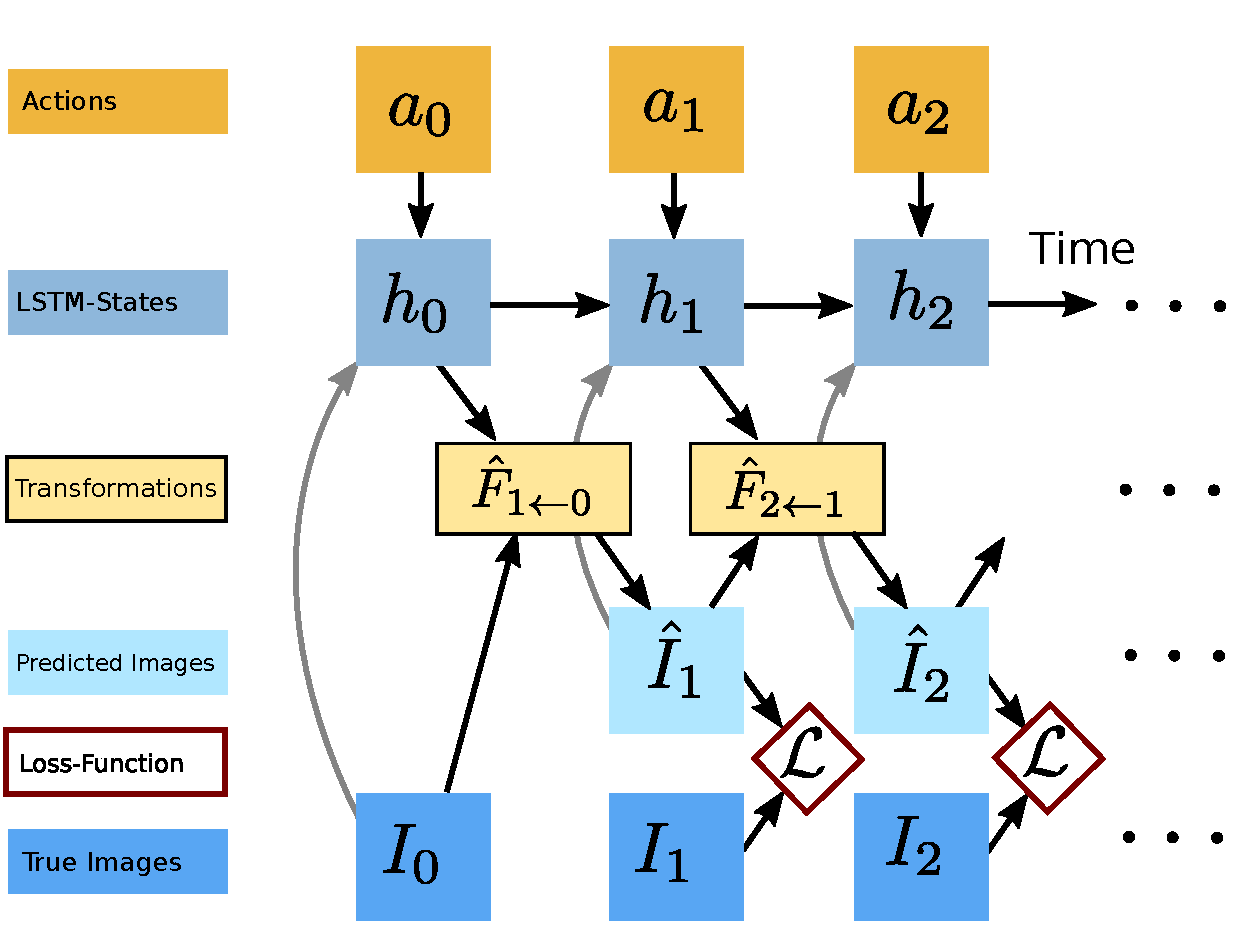
\includegraphics[width=0.7\columnwidth]{images_general/prediction_model.pdf}
	\caption{\small{Simplified structure of the video-prediction model. Time goes from left to right, $a_t$ are the actions, $h_t$ are the hidden states in the recurrent neural network, $\hat{F}_{t+1 \leftarrow t}$ is a 2D-warping field, $I_t$ are real images, and $\hat{I}_t$ are predicted images, $\mathcal{L}$ is a pairwise training-loss. \todo{update this}}}   
	\label{fig:prediction_model}
\end{figure}

In visual-MPC we use a transformation-based video-prediction architecture, first presented in \cite{finn_nips}. The advantage of using transformation based-models over a model that directly generates pixels, is that prediction is easier when only few objects in the image move by relatively small amounts and also the transformations can be leveraged to obtain predictions of \emph{where} certain pixels in the image are moving, a property that is used in several of our planning cost-function formulations. The model, which is implemented as a recurrent neural network $g_{\theta}$ parameterized by $\theta$, has a hidden state $h_t$ and takes in a previous image and an action at each step of the rollout. Future images $\hat{I}_{t+1}$ are generated by warping the previous generated image $\hat{I}_t$ or the previous true image $I_t$, when available, according to a 2-dimensional flow field $\hat{F}_{t+1 \leftarrow t}$. A simplifying illustration of model's structure is given in figure \ref{fig:prediction_model}. It is also summarized in the following two equations:

\begin{align}
[h_{t+1}, \hat{F}_{t+1 \leftarrow t}] 	&= g_{\theta}(a_t, h_t, I_t) \\
\hat{I}_{t+1} 							&= \hat{F}_{t+1 \leftarrow t} \diamond  \hat{I}_t 
\label{simple_dna}
\end{align}

Here bilinear sampling operator $\diamond$ interpolates the pixel values bilinearly with respect to a location $(x,y)$ and its four neighbouring pixels in the image, similar to \cite{zhou2016view}. Note that as shown in figure \ref{fig:prediction_model}, at the first time-step the real image is transformed, whereas at later timesteps previously generated images are transformed. The model is trained by standard backpropagtion-through time by performing gradient descent on a mean-squared error type image reconstruction loss, denoted by $\mathcal{L}$ in figure \ref{fig:prediction_model}.
\begin{figure}[t]
    \centering
    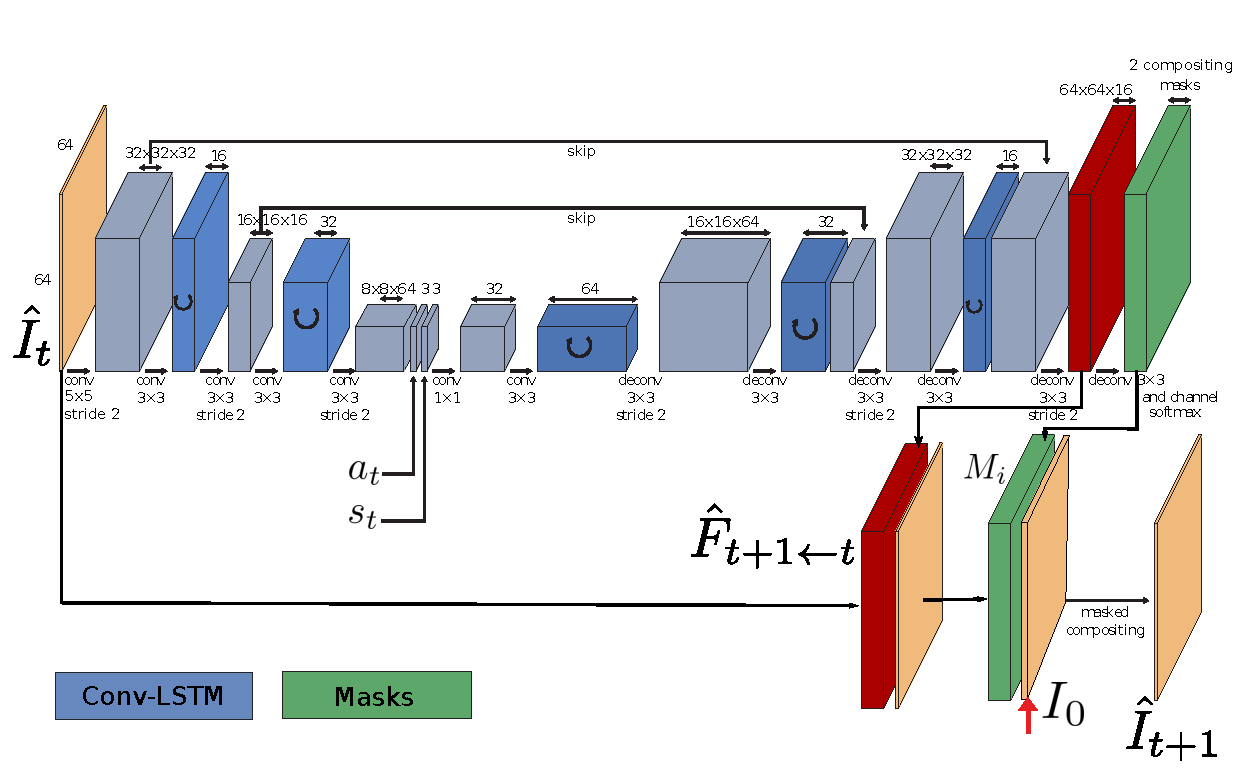
\includegraphics[width=\columnwidth]{images_sna/occlusionaware/architecture.pdf}
    \caption{\small{Forward pass through the recurrent SNA model based on \autoref{eqn:simplemodel}. The red arrow indicates where the image from the first time step $I_0$ is concatenated with the transformed images $\hat{F}_{t+1 \leftarrow t} \diamond  \hat{I}_t $ multiplying each channel with a separate mask to produce the predicted frame for step $t+1$.}}      \label{fig:occlusion_model}
\end{figure}

\label{subsec:pixel_trafo}
A forward pass of the RNN is illustrated in figure \ref{fig:occlusion_model}. We use a series stacked convolutional LSTMs and standard convolutional layers interleaved with average-pooling layers. The result of this computation is the 2 dimensional flow-field $\hat{F}_{t+1 \leftarrow t}$ which is used to transform a current image $I_t$ or $\hat{I}_t$.

\textbf{Predicting motion of individual pixels}: 
When using visual-MPC with a cost-function based on start- and goal pixel positions, a model is required that can effectively predict the 2-D motion of the user-selected start pixels $\pixel_0^{(1)}, \dots, \pixel_0^{(P)}$ up to $T$ steps into the future. Since the model we employ is transformation based, this motion prediction capability emerges implicitly, and therefore no external pixel motion supervision is required. To predict the future positions of the designated pixel $d$, the same transformations which are used to transform the images are applied to the distribution over designated pixel locations. The warping transformation $\hat{F}_{t+1 \leftarrow t}$ can be interpreted as a stochastic transition operator allowing us to make probabilistic predictions about future locations of individual pixels:

\begin{equation}
\hat{P}_{t+1} = \hat{F}_{t+1 \leftarrow t} \diamond  \hat{P}_t
\label{eqn:prob_forward}
\end{equation}

Here $P_t$ is a distribution over image locations which has the same spatial dimension as the image. For simplicity we assume that we only use a single designated pixel. At the first time step the distribution $\hat{P}_0$ is defined as 1 at the position of the user-selected designated pixel and zero elsewhere. The distribution $\hat{P}_{t+1}$ is normalized at each prediction step.

Since this basic model, which we refer to as dynamic neural advection (DNA) model, predicts images only based on the previous image, it is unable to recover shapes (e.g., objects) after they have been occluded, for example by the robot arm. Therefore, this model is only suitable for planning motions where the user-selected pixels are not occluded during the manipulation, which restricts its use in cluttered environments or with multiple selected pixels. In the next section, we introduce an enhanced type of model, which lifts this limitation by employing temporal skip connections.

Note that when using a planning cost function that does not depend on the prediction of pixel positions, like a classifier-based cost function, as detailed in section \ref{subsec:class_cost}, we do not require the model to output transformations and virtually any video prediction model can be used. 

\textbf{Skip Connection Neural Advection Model}
To enable effective tracking of objects through occlusions, we can extend the model discussed in the previous section with temporal skip connections: we now transform pixels not only from the previously generated image $\hat{I}_t$, but from all but from all previous images $\hat{I}_1,...\hat{I}_{t}$, including the context image $I_0$, which is a real image. All these transformed images can combined to a form the predicted image $\hat{I}_{t+1}$ by taking a weighted some over all transformed images, where the weights are given by masks $\mathbf{M}_t$ with the same size as the image and a single channel:
\begin{equation}
\hat{I}_{t+1} =  \mathbf{M}_{0} (\hat{F}_{t+1 \leftarrow 0} \diamond I_t) +  \sum_{j=1}^{\tau} \mathbf{M}_{j} (\hat{F}_{t+1 \leftarrow j} \diamond  \hat{I}_j).
\end{equation}

We refer to this model as the \emph{skip connection neural advection model (SNA)}, since it handles occlusions by using temporal skip-connections such that when a pixel is occluded (e.g., by the robot arm or by another object) it can still reappear later in the sequence.

Transforming from all previous images comes with increased computational cost, since the number of masks and transformations scales with the number of time-steps $\tau$. However, we found that in practice a greatly simplified version of this model, where transformations are applied only to the previous image and the \emph{first image} of the sequence $I_0$ works equally well. Moreover we found that transforming the first image of the sequence is not necessary, as the model uses its pixels primarily to generate the image background. Therefore, we can use the first image directly, without transformation, such that
\begin{equation}
\hat{I}_{t+1} = \mathbf{M}_{0} I_0 +  \mathbf{M}_{1} (\hat{F}_{t+1 \leftarrow t} \diamond \hat{I}_t).
\label{eqn:simplemodel}
\end{equation}
Here, we make the assumption that occluded objects are static throughout the prediction horizon. This assumption allows us to dispense the intermediate transformations and only provide a skip connection from the very first image in the sequence $I_0$, which is also the only real image, since all of the subsequent images are predicted by the model. Hence, this model only needs to output 2 masks. 

 \begin{wrapfigure}{r}{.37\columnwidth}
	\centering
	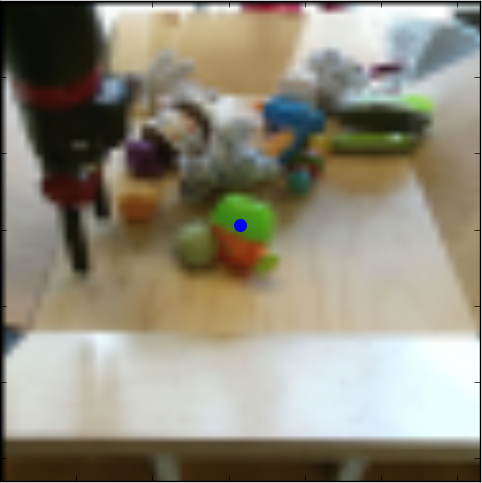
\includegraphics[width=0.37\columnwidth]{images_sna/occlusionaware/img_desigpixb0.png}
	\caption{The blue dot indicates the designated pixel}
	\label{fig:desig_pix_bluedot}
\end{wrapfigure}

We provide an example of the model recovering from occlusion in \autoref{fig:pix_reappear}. In this figure, the arm is predicted to move in front of the designated pixel, marked in blue in \autoref{fig:desig_pix_bluedot}. The predictions of the DNA model, shown in figure \autoref{fig:pix_reappear}(b), contain incorrect motion of the marked object, as shown in the heatmaps visualizing $\hat{P}_t$, although the arm actually passes in front of it. This is because the DNA model cannot recover information about an object that it has `overwritten' during its predictions, causing the model to predict that the pixel \emph{moves with the arm}. We identified this as one of the major causes of planning failure using the DNA model. By contrast our SNA model predicts that the occluded object will not move, shown in figure  \autoref{fig:pix_reappear}(a).

%\todo{can cut from here:}
%Next, we show another illustration comparing the occlusion handling of DNA and the proposed SNA model. The graphs in \autoref{fig:pix_reqppear_graph} show the predicted probability evaluated at the position of the designated pixel, shown in figure \ref{fig:desig_pix_bluedot}, which is stationary during the entire motion. Precisely when the arm occludes the designated pixel, the probability at this point decreases. This indicates that the model is `unsure' where this pixel is. When the arm unoccludes the designated pixel, it should become visible again, and the probability of the designated pixel being at its original position should go up. In the case of the DNA model and its variants~\cite{finn_nips}, the probability mass does not increase after the object reappears. 
% 
% \begin{figure}[t]
% 	\centering
% 	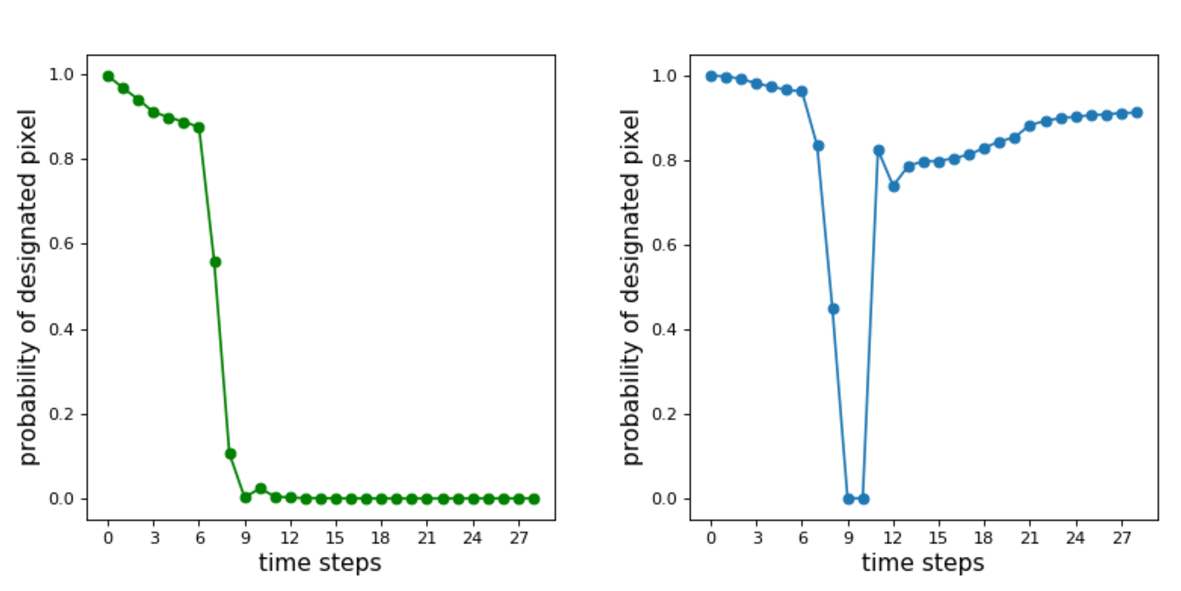
\includegraphics[width=0.9\columnwidth]{images_sna/occlusionaware/probability_curves.pdf}
% 	\caption{Predicted probability $P_{d^{(0)}}(t)$ of the designated pixel being at the location of the blue dot indicated in \autoref{fig:desig_pix_bluedot} for the DNA model (left) and the SNA model (right). \todo{can cut if no more space!}}      \label{fig:pix_reqppear_graph}
% \end{figure}

\begin{figure}
    \centering
    \begin{subfigure}{0.9\columnwidth}
    \centering
        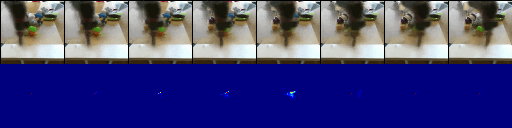
\includegraphics[width=1.\linewidth]{images_sna/occlusionaware/cdna_1ststep_bckgd_gen_pixb0_overtime.png}
        \caption{Skip connection neural advection (SNA) does not erase or move objects in the background}
        \label{fig:Ng1}
    \end{subfigure}
    \begin{subfigure}{0.9\columnwidth}
    \centering
        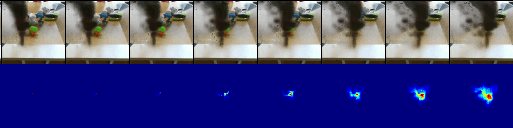
\includegraphics[width=1.0\linewidth]{images_sna/occlusionaware/orig_dna_gen_pixb0_overtime.png}
        \caption{Standard DNA \cite{foresight} exhibits undesirable movement of the distribution $P_{d}(t)$ and erases the background}
    \end{subfigure}
    \caption{
    %\protect\subref{fig:Ng1} 
    Top rows: Predicted images of arm moving \textit{in front of} green object with designated pixel (as indicated in \autoref{fig:desig_pix_bluedot}). 
    %(\protect\subref{fig:Ng2}) 
    Bottom rows: Predicted probability distributions $P_{d}(t)$ of designated pixel obtained by repeatedly applying transformations.}
    \label{fig:pix_reappear}
\end{figure}

% explain evolution of video-predction models, CDNA, SNA, SAVP

\section{Planning Cost Functions}
\label{sec:cost}
In this section we present three different kinds of goal specification mechanisms and cost functions that may be used for planning with visual MPC, and discuss their tradeoffs.

\edit{
One na\"{i}ve approach for the cost function could be to use the pixel-wise error, such as MSE, between a \emph{goal image} and the \emph{predicted image}. However there is a severe issue with this approach: Large objects in the image such as the arm would dominate the cost, therefore a common failure mode is that the planner matches the position of the arm with the position in the goal image, ignoring the smaller objects.}

\subsection{Pixel-Distance Cost}
\label{subsec:pixel_dist_cost}
A convenient way to define a robot task is by choosing one or more pixels in the robot's camera view and choosing a destination where each pixel should be moved. For example, the user might select a pixel on an object and ask the robot to move it 10 cm to the left. \edit{This type of objective is general, in that it can define any object relocation task, while being easy to specify by  the user through clicks. Also success can be measured quantitatively in a straight-forward way, as detailed in section \ref{sec:experiments}.}
 
Given a distribution over pixel positions $P_0$ at time $t = 0$, our model predicts distributions over its positions $P_t$ at time $t \in \{ 1, \dots, T \}$. One way of defining the cost per time-step $c_t$ is by using the expected Euclidean distance to the goal point $d_g$, which is straight-forward to calculate from $P_t$ and $g$, as follows:
 \begin{align}
c = \sum_{t = 1, \dots, T} c_t =  \sum_{t = 1, \dots, T} \mathbb{E}_{\hat{d}_{t} \sim P_{t}} \left[\|\hat{d}_{t} - d_{g}\|_2\right] 
 \label{eq:cost}
 \end{align}
The per time-step costs $c_t$ are summed together giving the overall planing objective $c$. The expected distance to the goal provides a smooth planning objective and enables longer-horizon tasks, since this cost function encourages movement of the designated objects into the right direction for each step of the execution, regardless of whether the goal-position can be reached within $T$ time steps or not. This cost also makes use of the uncertainty estimates of the predictor, when computing the expected distance to the goal. For multi-objective tasks with multiple designated pixels $d^{(i)}$ the costs are summed to together, and optionally weighted according to a scheme discussed in \autoref{subsec:reg_cost}.  

\subsection{Registration-Based Cost}
\label{subsec:reg_cost}
\edit{When using pixel distance-based cost functions it is necessary to know the \emph{current} location of the object,  $\pixel_0^{(1)}, \dots, \pixel_0^{(P)}$ at each time-step, so that the model can predict the positions of this particular pixel from the current step forward.}
To update the belief of where the target object currently is, we register the current image to the start and optionally also to a \emph{goal image}, where the designated pixels are marked by the user. Adding a goal-image can make visual MPC more precise, since when the target object is close to the goal position, registration to the goal-image greatly improves the position estimate of the designated pixel. Crucially, the registration method we introduce is self-supervised, using the same exact data for training the video prediction model and the registration model. This allows both the predictor and registration model to continuously improve as the robot collects more data.

\begin{figure}
	\centering
	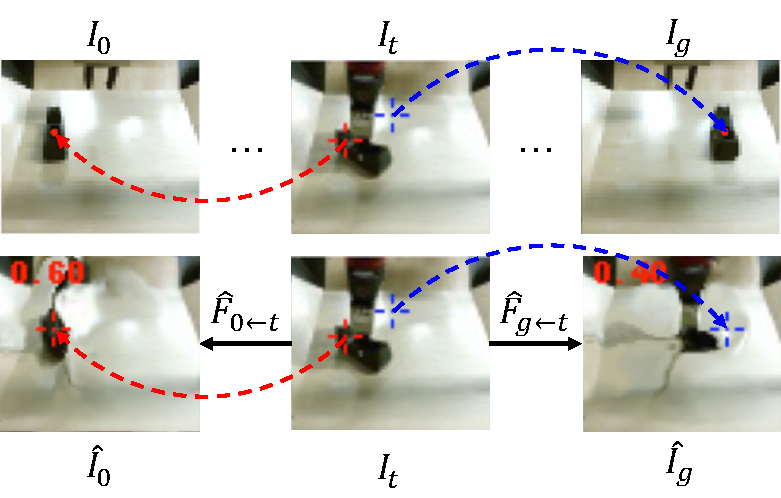
\includegraphics[width=0.8\linewidth]{images_rfr/registration_singletime.pdf}
	\vspace{-0.3cm}
	\caption{\small{Closed loop control is achieved by registering the current image $I_t$ globally to the first frame $I_0$ and the goal image $I_g$. In this example registration to $I_0$ succeeds while registration to $I_g$ fails since the object in $I_g$ is too far away.}
		\label{fig:reg_single}
	}
\end{figure}

\noindent \textbf{Test Time Procedure}
We will first describe the registration scheme at test time (see Figure~\ref{fig:registration_arch}(a)). We separately register the current image $I_t$ to the start image $I_0$ and to the goal image $I_g$ by passing it into the registration network $R$, implemented as a fully-convolutional neural network. The registration network produces a flow map $\hat{F}_{0 \leftarrow t} \in \mathbb{R}^{H \times W \times 2}$, a vector field with the same size as the image, that describes the relative motion for every pixel between the two frames.
\begin{align}
\hat{F}_{0 \leftarrow t} = R(I_t, I_0) &&
\hat{F}_{g \leftarrow t} = R(I_t, I_g)
\end{align}
The flow map $\hat{F}_{0 \leftarrow t}$ can be used to warp the image of the current time step $t$ to the start image $I_0$, and $\hat{F}_{g \leftarrow t}$ can be used to warp from $I_t$ to $I_g$ (see Figure \ref{fig:reg_single} for an illustration). There is no difference to the warping operation used in the video-prediction model, explained in section \ref{sec:model}, equation \ref{simple_dna}:
\begin{align}
\hat{I}_0 = \hat{F}_{0 \leftarrow t} \diamond  I_t &&
\hat{I}_g = \hat{F}_{g \leftarrow t} \diamond  I_t 
\end{align}
In essence for a current image $\hat{F}_{0 \leftarrow t}$ puts $I_t$ in correspondence with $I_0$, and $\hat{F}_{g \leftarrow t}$ puts $I_t$ in correspondence with $I_g$. The motivation for registering to both $I_0$ and $I_g$ is to increase accuracy and robustness. In principle, registering to either $I_0$ or $I_g$ is sufficient.

While the registration network is trained to perform a global registration between the images, we only evaluate it at the points $d_0$ and $d_g$ chosen by the user. This results in a cost function that ignores distractors. The flow map produced by the registration network is used to find the pixel locations corresponding to $d_0$ and $d_g$ in the current frame: 
\begin{align}
\hat{d}_{0,t} = d_0 + \hat{F}_{0 \leftarrow t}(d_0) &&
\hat{d}_{g,t} = d_g + \hat{F}_{g \leftarrow t}(d_g)
\label{eqn:warped_pos}
\end{align}


\begin{figure}[t!]
	\centering
	\begin{subfigure}[b]{0.35\linewidth}
		\centering
		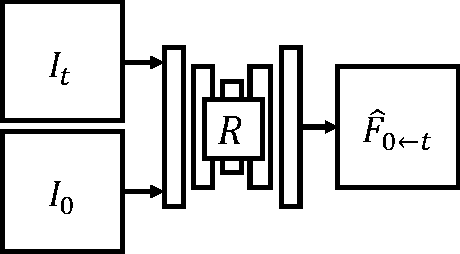
\includegraphics[width=\linewidth]{images_rfr/registration_test_start.pdf}\vspace{2.5mm}
		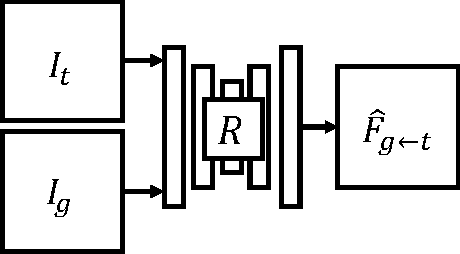
\includegraphics[width=\linewidth]{images_rfr/registration_test_goal.pdf}
		\caption{\small{Testing usage.}}
	\end{subfigure}
	\quad \quad
	\begin{subfigure}[b]{0.55\linewidth}
		\centering
		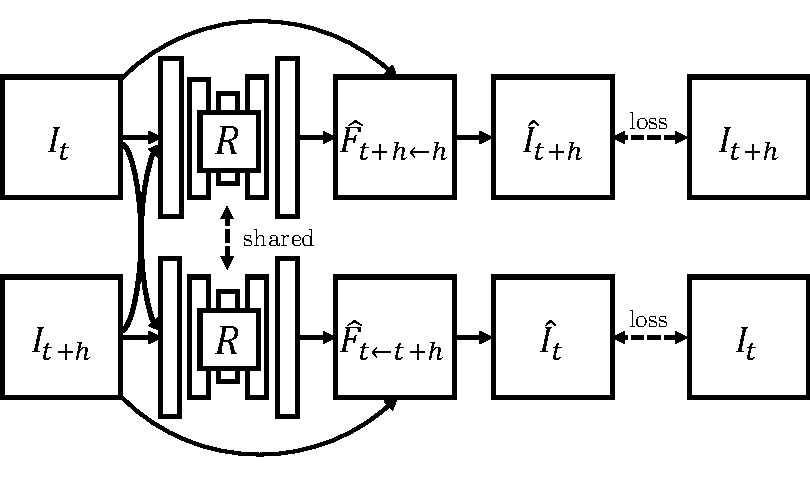
\includegraphics[width=\linewidth,trim={0 3mm 0 3mm},clip]{images_rfr/registration_train.pdf}
		\caption{\small{Training usage.}}
		\label{fig:discrete}
	\end{subfigure}
	\vspace{-1mm}
	\caption{\small{(a) At test time the registration network registers the current image $I_t$ to the start image $I_0$ (top) and goal image $I_g$ (bottom), inferring the flow-fields $\hat{F}_{0 \leftarrow t}$ and $\hat{F}_{g \leftarrow t}$. (b) The registration network is trained by warping images from randomly selected timesteps along a trajectory to each other.
	}}
	\label{fig:registration_arch}
\end{figure}

\begin{figure*}
	\centering
	\vspace{-0.1in}	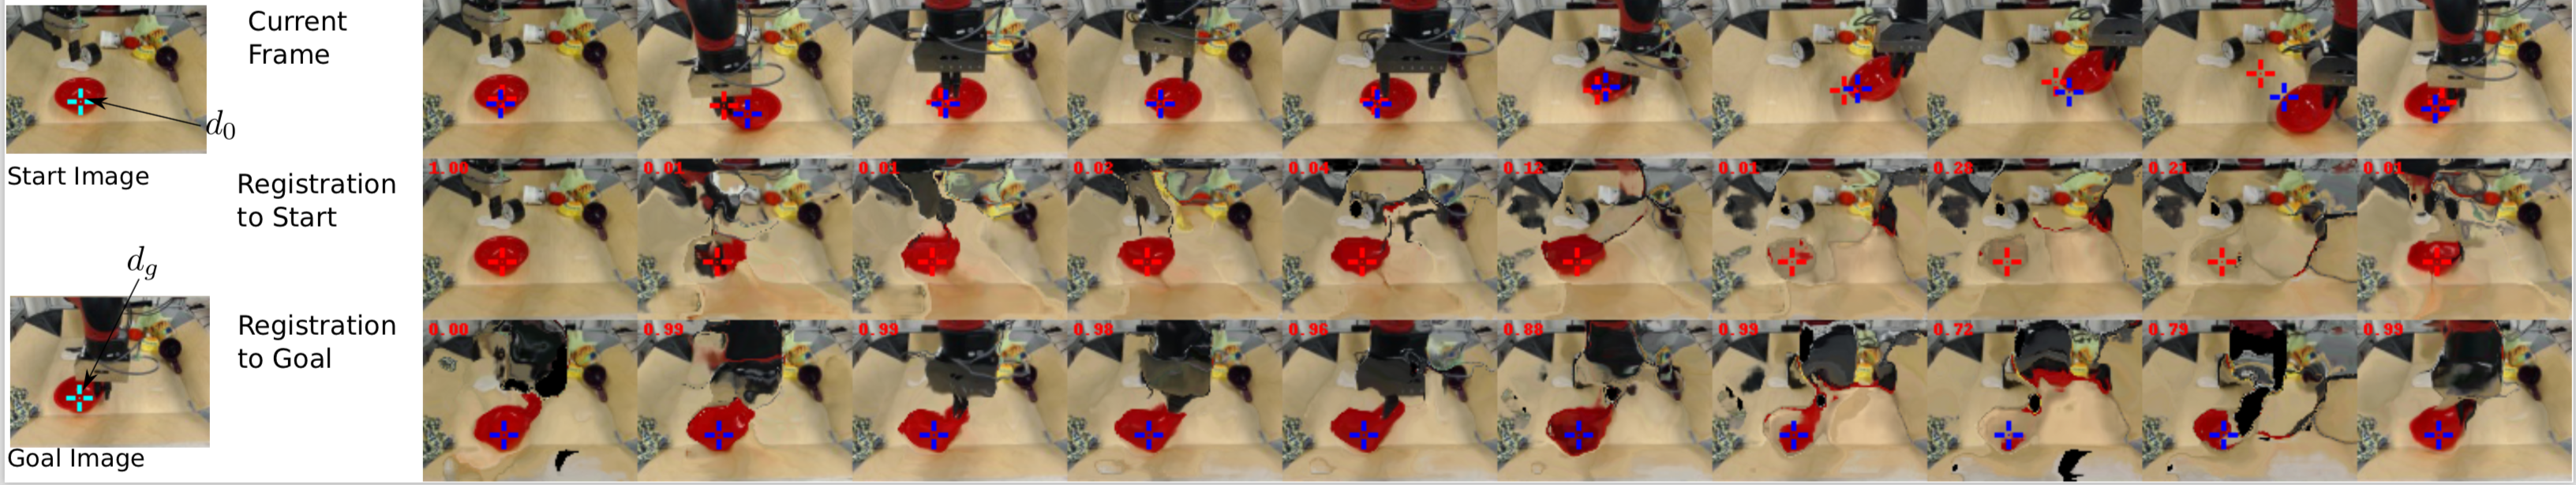
\includegraphics[width=1\linewidth]{images_rfr/reg_over_time.png}
	\caption{\small{Outputs of registration network. The first row shows the timesteps from left to right of a robot picking and moving a red bowl, the second row shows each image warped to the initial image via registration, and the third row shows the same for the goal image. A successful registration in this visualization would result in images that closely resemble the start- or goal image. In the first row, the locations where the designated pixel of the start image $d_0$ and the goal image $d_g$ are found are marked with red and blue crosses, respectively. It can be seen that the registration to the start image (red cross) is failing in the second to last time step, while the registration to the goal image (blue cross) succeeds for all time steps. The numbers in red, in the upper left corners indicate the trade off factors $\lambda$ between the views and are used as weighting factors for the planning cost. (Best viewed in PDF)}}
	\label{fig:tracking_overtime}
	\vspace{-0.2in}
\end{figure*}

For simplicity, we describe the case with a single designated pixel. In practice, instead of a single flow vector $\hat{F}_{0 \leftarrow t}(d_0)$ and $\hat{F}_{g \leftarrow t}(d_g)$, we consider a neighborhood of flow-vectors around $d_0$ and $d_g$ and take the median in the $x$ and $y$ directions, making the registration more stable.
\autoref{fig:tracking_overtime} visualizes an example tracking result while the gripper is moving an object.

\noindent \textbf{Registration-Based Pixel-Distance Cost}
Registration can fail when distances between objects in the images are large. During a motion, the registration to the first image typically becomes harder, while the registration to the goal image becomes easier. We propose a mechanism that estimates which image is registered correctly, allowing us to utilize only the successful registration for evaluating the planning cost. This mechanism gives a high weight $\lambda_i$ to pixel-distance costs $c_i$ associated with a designated pixel $\hat{d}_{i,t}$ that is tracked successfully and a low, ideally zero, weight to a designated pixel where the registration is poor. We use the photometric distance between the true frame and the warped frame evaluated at $d_{0,i}$ and $d_{g,i}$ as an estimate for \emph{local} registration success. A low photometric error indicates that the registration network predicted a flow vector leading to a pixel with a similar color, thus indicating warping success. However this does not necessarily mean that the flow vector points to the correct location. For example, there could be several objects with the same color and the network could simply point to the wrong object. Letting $I_i(d_i)$ denote the pixel value in image $I_i$ for position $d_i$, and $\hat{I}_i(d_i)$ denote the corresponding pixel in the image warped by the registration function, we can define the general weighting factors $\lambda_i$ as:
\begin{align}
\lambda_i =  \frac{||I_i(d_i) - \hat{I_i}(d_i)||_2^{-1}}{\sum^N_j ||I_j(d_j) - \hat{I}_j(d_j)||^{-1}_2}.
\label{eqn:cost_avg}
\end{align}
where $\hat{I}_i = \hat{F}_{i \leftarrow t} \diamond I_t$. The MPC cost is computed as the average of the costs $c_i$ weighted by $\lambda_i$, where each $c_i$ is the expected distance (see equation \ref{eq:cost}) between the registered point $\hat{d}_{i,t}$ and the goal point $d_{g,i}$. Hence, the cost used for planning is $c = \sum_i \lambda_i c_i$.  In the case of the single view model and a single designated pixel, the index $i$ iterates over the start and goal image (and $N=2$).

The proposed weighting scheme can also be used with multiple designated pixels, as used in multi-task settings and multi-view models, which are explained in section \ref{sec:multiview}. The index $i$ then also loops over the views and indices of the designated pixels.

\noindent \textbf{Training Procedure}
The registration network is trained on the same data as the video-prediction model, but it does not share parameters with it.\footnote{In principle, sharing parameters with the video-prediction model might be beneficial, but this is left for future work.} Our approach is similar to the optic flow method proposed by \cite{meister2017unflow}. However, unlike this prior work, our method computes registrations for frames that might be many time steps apart, and the goal is not to extract optic flow, but rather to determine correspondences between potentially distant images. For training, two images are sampled at random times steps $t$ and $t+h$ along the trajectory and the images are warped to each other in both directions. 
\begin{align}
\hat{I}_{t} = \hat{F}_{t \leftarrow t +h} \diamond  I_{t+h} &&
\hat{I}_{t+h} = \hat{F}_{t+h \leftarrow t} \diamond  I_{t}
\end{align}
The network, which outputs $\hat{F}_{t \leftarrow t +h}$ and $\hat{F}_{t+h \leftarrow t}$, see Figure~\ref{fig:registration_arch} (b), is trained to minimize the photometric distance between $\hat{I}_t$ and $I_t$ and $\hat{I}_{t+h}$ and $I_{t+h}$, in addition to a smoothness regularizer that penalizes abrupt changes in the outputted flow-field. The details of this loss function follow prior work \cite{meister2017unflow}. We found that gradually increasing the temporal distance $h$ between the images during training yielded better final accuracy, as it creates a learning curriculum. The temporal distance is linearly increased from 1 step to 8 steps at 20k SGD steps. In total 60k iterations were taken.

The network $R$ is implemented as a fully convolutional network taking in two images stacked along the channel dimension. First the inputs are passed into three convolutional layers each followed by a bilinear downsampling operation. This is passed into three layers of convolution each followed by a bilinear upsampling operation (all convolutions use stride 1). By using bilinear sampling for increasing or decreasing image sizes we avoid artifacts that are caused by strided convolutions and deconvolutions.


\subsection{Classifier-Based Cost Functions}
\label{subsec:class_cost}
An alternative way to define the cost function is with a goal classifier. This type of cost function is particularly well-suited for tasks that can be completed in multiple ways. For example, for a task of rearranging a pair objects into relative positions, i.e. pushing the first object to the left of the second object, the absolute positions of the objects do not matter nor does the arm position. A classifier-based cost function allows the planner to discover any of the possible goal states. 

Unfortunately, a typical image classifier will require a large amount of labeled examples to learn, and we don't want to collect large datasets for each and every task. Instead, we aim to learn a goal classifier from only a few positive examples, using a meta-learning approach. A few positive examples of success are easy for people to provide and are the minimal information needed to convey a goal.

\newcommand{\task}{\mathcal{T}}
\newcommand{\data}{\mathcal{D}}
\newcommand{\obs}{\mathbf{o}}
\newcommand{\out}{y}
\newcommand{\posdata}{\data^+}
\newcommand{\testdata}{\data^\text{test}}
\newcommand{\loss}{\mathcal{L}}

Formally, we consider a goal classifier $\hat{\out} = f(\obs)$, where $\obs$ denotes the image observation, and $\hat{\out} \in [0,1]$ indicates the predicted probability of the observation being of a successful outcome of the task. Our objective is to infer a classifier for a new task $\task_j$ from a few positive examples of success, which are easy for a user to provide and encode the minimal information needed to convey a task. In other words, given a dataset $\posdata_j$ of $K$ examples of successful end states for a new task $\task_j$: $\data_j:=\{(\obs_k, 1) | k = 1...K\}_j$, our goal is to infer a classifier for task $\task_j$. 

\begin{figure}
    \centering
    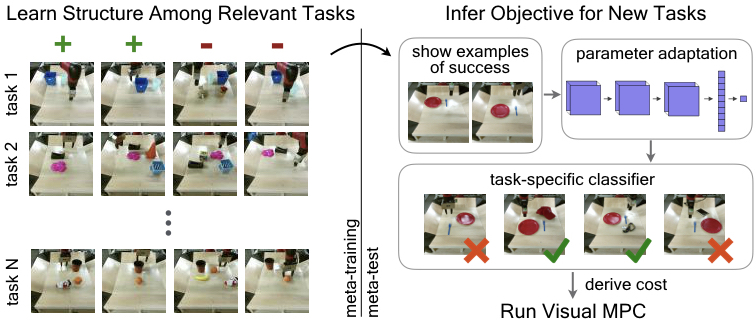
\includegraphics[width=1.0\columnwidth]{images_cls/cls_fig_2.jpeg}
    \caption{\small We propose a framework for quickly specifying visual goals. Our goal classifier is meta-trained with positive and negative examples for diverse tasks (left), which allows it to meta-learn that some factors matter for goals (e.g., relative positions of objects), while some do not (e.g. position of the arm). At meta-test time, this classifier can learn goals for new tasks from a few of examples of success (right - the goal is to place the fork to the right of the plate). The cost can be derived from the learned goal classifier for use with visual MPC.}
    \label{fig:cls_fig}
    \vspace{-0.3cm}
\end{figure}

\noindent \textbf{Meta-Learning for Few-Shot Goal Inference:}
To solve the above problem, we propose learning a few-shot classifier that can infer the goal of a new task from a small set of goal examples, allowing the user to define a task from a few examples of success. To train the few-shot classifier, we first collect a dataset of both positive and negative examples for a wide range of tasks. We then use this data to learn how to learn goal classifiers from a few positive examples.
Our approach is illustrated in Figure~\ref{fig:cls_fig}.

We build upon model-agnostic meta-learning (MAML)~\cite{maml}, which learns initial parameters $\theta$ for model $f$ that can efficiently adapt to a new task with one or a few steps of gradient descent. Grant et al. \cite{caml} proposed an extension of MAML, referred to as concept acquisition through meta-learning (CAML), for learning to learn new concepts from positive examples alone. We apply CAML to the setting of acquiring goal classifiers from positive examples, using a meta-training data with both positive and negative examples. The result of the meta-training procedure is an initial set of parameters that can be used to learn new goal classifiers at test time.

\noindent \textbf{Test Time Procedure:}
At test time, the user provides a dataset $\posdata_j$ of $K$ examples of successful end states for a new task $\task_j$: $\data_j:=\{(\obs_k, 1) | k = 1...K\}_j$, which are then used to infer a task-specific goal classifier $C_j$. In particular, the meta-learned parameters $\theta$ are updated through gradient descent to adapt to task $\task_j$:

$$
C_j(\obs)
= f(\obs; \theta_j')
= f\big(\obs; \theta-\alpha \nabla_\theta \!\!\! \sum_{(\obs_n, \out_n)\in \posdata_j} \loss (\out_n, f(\obs_n; \theta)\big)
$$

where $\loss$ is the cross-entropy loss function, $\alpha$ is the step size, and $\theta'$ denotes the parameters updated through gradient descent on task $\task_j$.

During planning, the learned classifier $C_j$ takes as input an image generated by the video-prediction model and outputs the predicted probability of the goal being achieved for the task specified by the few examples of success. To convert this into a cost function, we treat the probability of success as the planning cost for that observation. To reduce the effect of false positives and mis-calibrated predictions, we use the classifier conservatively by thresholding the predictions so that reward is only given for confident successes. Below this threshold, we give a reward of 0 and above this threshold, we provide the predicted probability as the reward.


\noindent \textbf{Training time procedure}
During meta-training, we explicitly train for the ability to infer goal classifiers for the set of training tasks, $\{ \task_i \}$. We assume a small dataset $\data_i$ for each task $\task_i$, consisting of both positive and negative examples: $\data_i:= \{(\obs_n,\out_n) | n=1...N \}_i$. To learn the initial parameters $\theta$, we optimize the following objective using Adam~\cite{ADAM}:

$$
\min_\theta \sum_i \sum_{(\obs_n, y_n) \in \testdata_i} \loss(\out_n, f(\obs_n; \theta_i')) 
$$

In our experiments, our classifier is represented by a convolutional neural network, consisting of three convolutional layers, each followed by layer normalization and a ReLU non-linearity. After the final convolutional layer, a spatial soft-argmax operation extracts spatial feature points, which are then passed through fully-connected layers.

\subsection{When to Use Which Cost Function?}
\label{subsec:cost_discuission}

We have introduced three different kinds of cost functions, pixel-distance based cost functions with and without registration, as well as classifier-based cost functions. Here we discuss the relative strengths and weaknesses of each of them.

Pixel-distance based cost functions have the advantage that they allow moving objects precisely to target locations. They are also easy to specify, without requiring any images or examples, and therefore provide an easy and fast user interface. The pixel-distance based cost function also has a high degree of robustness against distractor objects and clutter, since the optimizer can ignore the values of other pixels; this is important when targeting diverse real-world environments.
By incorporating an image of the goal, we can also add a registration mechanism to allow for more robust closed-loop control, at the cost of a more significant burden on the user.

The classifier-based cost function allows for solving more abstract tasks where the absolute positions of an object is not relevant, such as positioning a cup in front of a plate, irrespective of where the plate is.  Providing a few example images takes more effort than specifying pixel locations but allows a broader range of goal sets to be specified.


% pixel distance based costs
% registration based costs
% combination of registration based cost with pixel distance cost
% classifier based costs

\section{Trajectory Optimizer}
\label{sec:optimizer}

%%SL.10.15: It's bad form to begin a technical section with prior work. Prior work belongs in the related work section.
Prior work has also proposed to plan through learned models via differentiation, though not with visual inputs~\cite{deep_mpc}. We instead use a stochastic, sampling-based trajectory optimization method~\cite{cem-rk-13,foresight}, which we extend to handle a mixture of continuous and discrete actions.

The role of the optimizer is to find actions sequences $a_{1:T}$ which minimize the sum of the costs $c_{1:T}$ along the planning horizon $T$. This is achieved via iterative sampling using the Cross-Entropy Method
%%SL.10.15: algorithm names are not capitalized
and ranking of each video-prediction rollout using a cost function. 

In the model-predictive control setting, the action sequences found by the optimizer can be very different between execution real-world times steps. For example at one time step the optimizer might find a pushing action leading towards the goal and in the next time step it determines a grasping action to be optimal to reach the goal. Na\"{i}ve replanning at every time step can then result in alternating between a pushing and a grasping attempt indefinitely causing the agent to get stuck and not making any progress towards to goal. 

%%SL.10.15: It's not clear whether this is done in every experiment or just some experiments.
We can resolve this problem by modifying the sampling distribution of the first iteration of CEM so that the optimizer commits to the plan found in the previous time step. In prior work \cite{sna}
%%SL.10.15: that's not really prior work for this paper...
the sampling distribution at first iteration of CEM is chosen to be a Gaussian with diagonal covariance matrix and zero mean. We instead use the best action sequence found in the optimization of the \emph{previous} real-world time step as the mean for sampling new actions in the \emph{current} real-world time-step. Since this action sequence is optimized for the previous time step we only use the values $a_{2:T}$ and omit the first action. To sample actions close to the action sequence from the previous time step we reduce the entries of the diagonal covariance matrix for the first $T-1$ time steps. It is crucial that the last entry of the covariance matrix at the end of the horizon is not reduced otherwise no exploration could happen for the last time step causing poor performance at later time steps.
% explain the cross entroy method
% explain reusing actions

\section{Custom Action Sampling Distributions}

\label{sec:system}
When collecting data by sampling from simple distributions, such as a multivariate Gaussian, the skills that emerged were found to be generally restricted to pushing and dragging objects. This is because with simple distributions, it is very unlikely to visit states like picking up and placing of objects or folding cloth. Not only would the model be imprecise for these kinds of states, but also during planning it would be unlikely to \emph{find} action sequences that grasp an object or fold a piece of cloth. 
We therefore explore how the sampling distribution used both in data collection and sampling-based planning can be changed to visit these, otherwise unlikely, states more frequently, allowing more complex behavior to emerge. 

\noindent \textbf{Learning Pick and Place Behavior:}
We first discuss picking and placing of objects. To allow picking up and placing of objects to occur more frequently, we incorporate a simple ``reflex'' during data collection, where the gripper automatically closes, when the height of the wrist above the table is lower than a small threshold. This reflex is inspired by the palmar reflex observed in infants~\cite{grasping_fetal}. With this primitive, about 20\% of training trajectories included some sort of grasp on an object. It is worth noting that, other than this reflex, no grasping-specific engineering was applied to the policy, allowing a joint pushing and grasping policy to emerge through planning (see figure \ref{fig:push_grasp} in the appendix). In our experiments, we evaluate our method using data obtained both with and without the grasping reflex, evaluating both purely non-prehensile and combined prehensile and non-prehensile manipulation.

\noindent \textbf{Learning Deformable Object Manipulation:}
In order to collect meaningful interaction data for learning folding of deformable objects such as towels and cloths, we adapted the sampling distribution to increase the likelihood of encountering ``cloth-folding-states`` in the data. When using actions sampled from a simple distribution or the previously-described distribution, cloths would become tangled and we would see many ``sweeping motions``. To improve the efficiency of encountering ``cloth folds``, we use the same action primitive used both for grasping primitive, but additionally we reduce lateral motion of the end-effector when the gripper is close to the table, thus reducing the undesired ``sweeping motions``.
%%SL.10.15: Have transition here and explain what this section is about. Currently, it seems like a bunch of disjointed miscallaneous stuff that didn't fit in anywhere else. This is not good. Maybe you can call this system design and describe the robot setup here first (both single view and multi-view), then details about data collection -- how actions are selected etc. (which can be merged with 7.2). Figures would help to illustrate the robot setup. 7.3 probably doesn't belong here at all, but belongs in experiments

Further details about the data collection process can be found in section \ref{sec:experiment_setup} in the appendix.

\section{Multi-View Visual MPC}
\label{sec:multiview}
The visual MPC algorithm as described so far is only able to solve manipulation tasks specified in 2D, like rearranging objects on the table. However, this can impose severe limitations; for example, a task such as lifting an object to a particular position in 3D cannot be fully specified with a single view, since it would be ambiguous. 

We use a combination of two views, taken from two cameras arranged appropriately, to jointly define a 3D task. Figure \ref{fig:robot_setup} shows the robot setup, including two standard webcams observing the workspace from different angles. The registration method described in the previous section is used separately per view to allow for dynamic retrying and solving temporally extended tasks. The planning costs from each view are combined using weighted averaging where the weights are provided by the registration network (see equation \ref{eqn:cost_avg}).  The the first two rows of figure \ref{fig:tile_2} show a "placing task" specified in two views, where an object needs 







\section{Experimental Evaluation}
\begin{wrapfigure}{r}{.45\columnwidth}
	\centering
	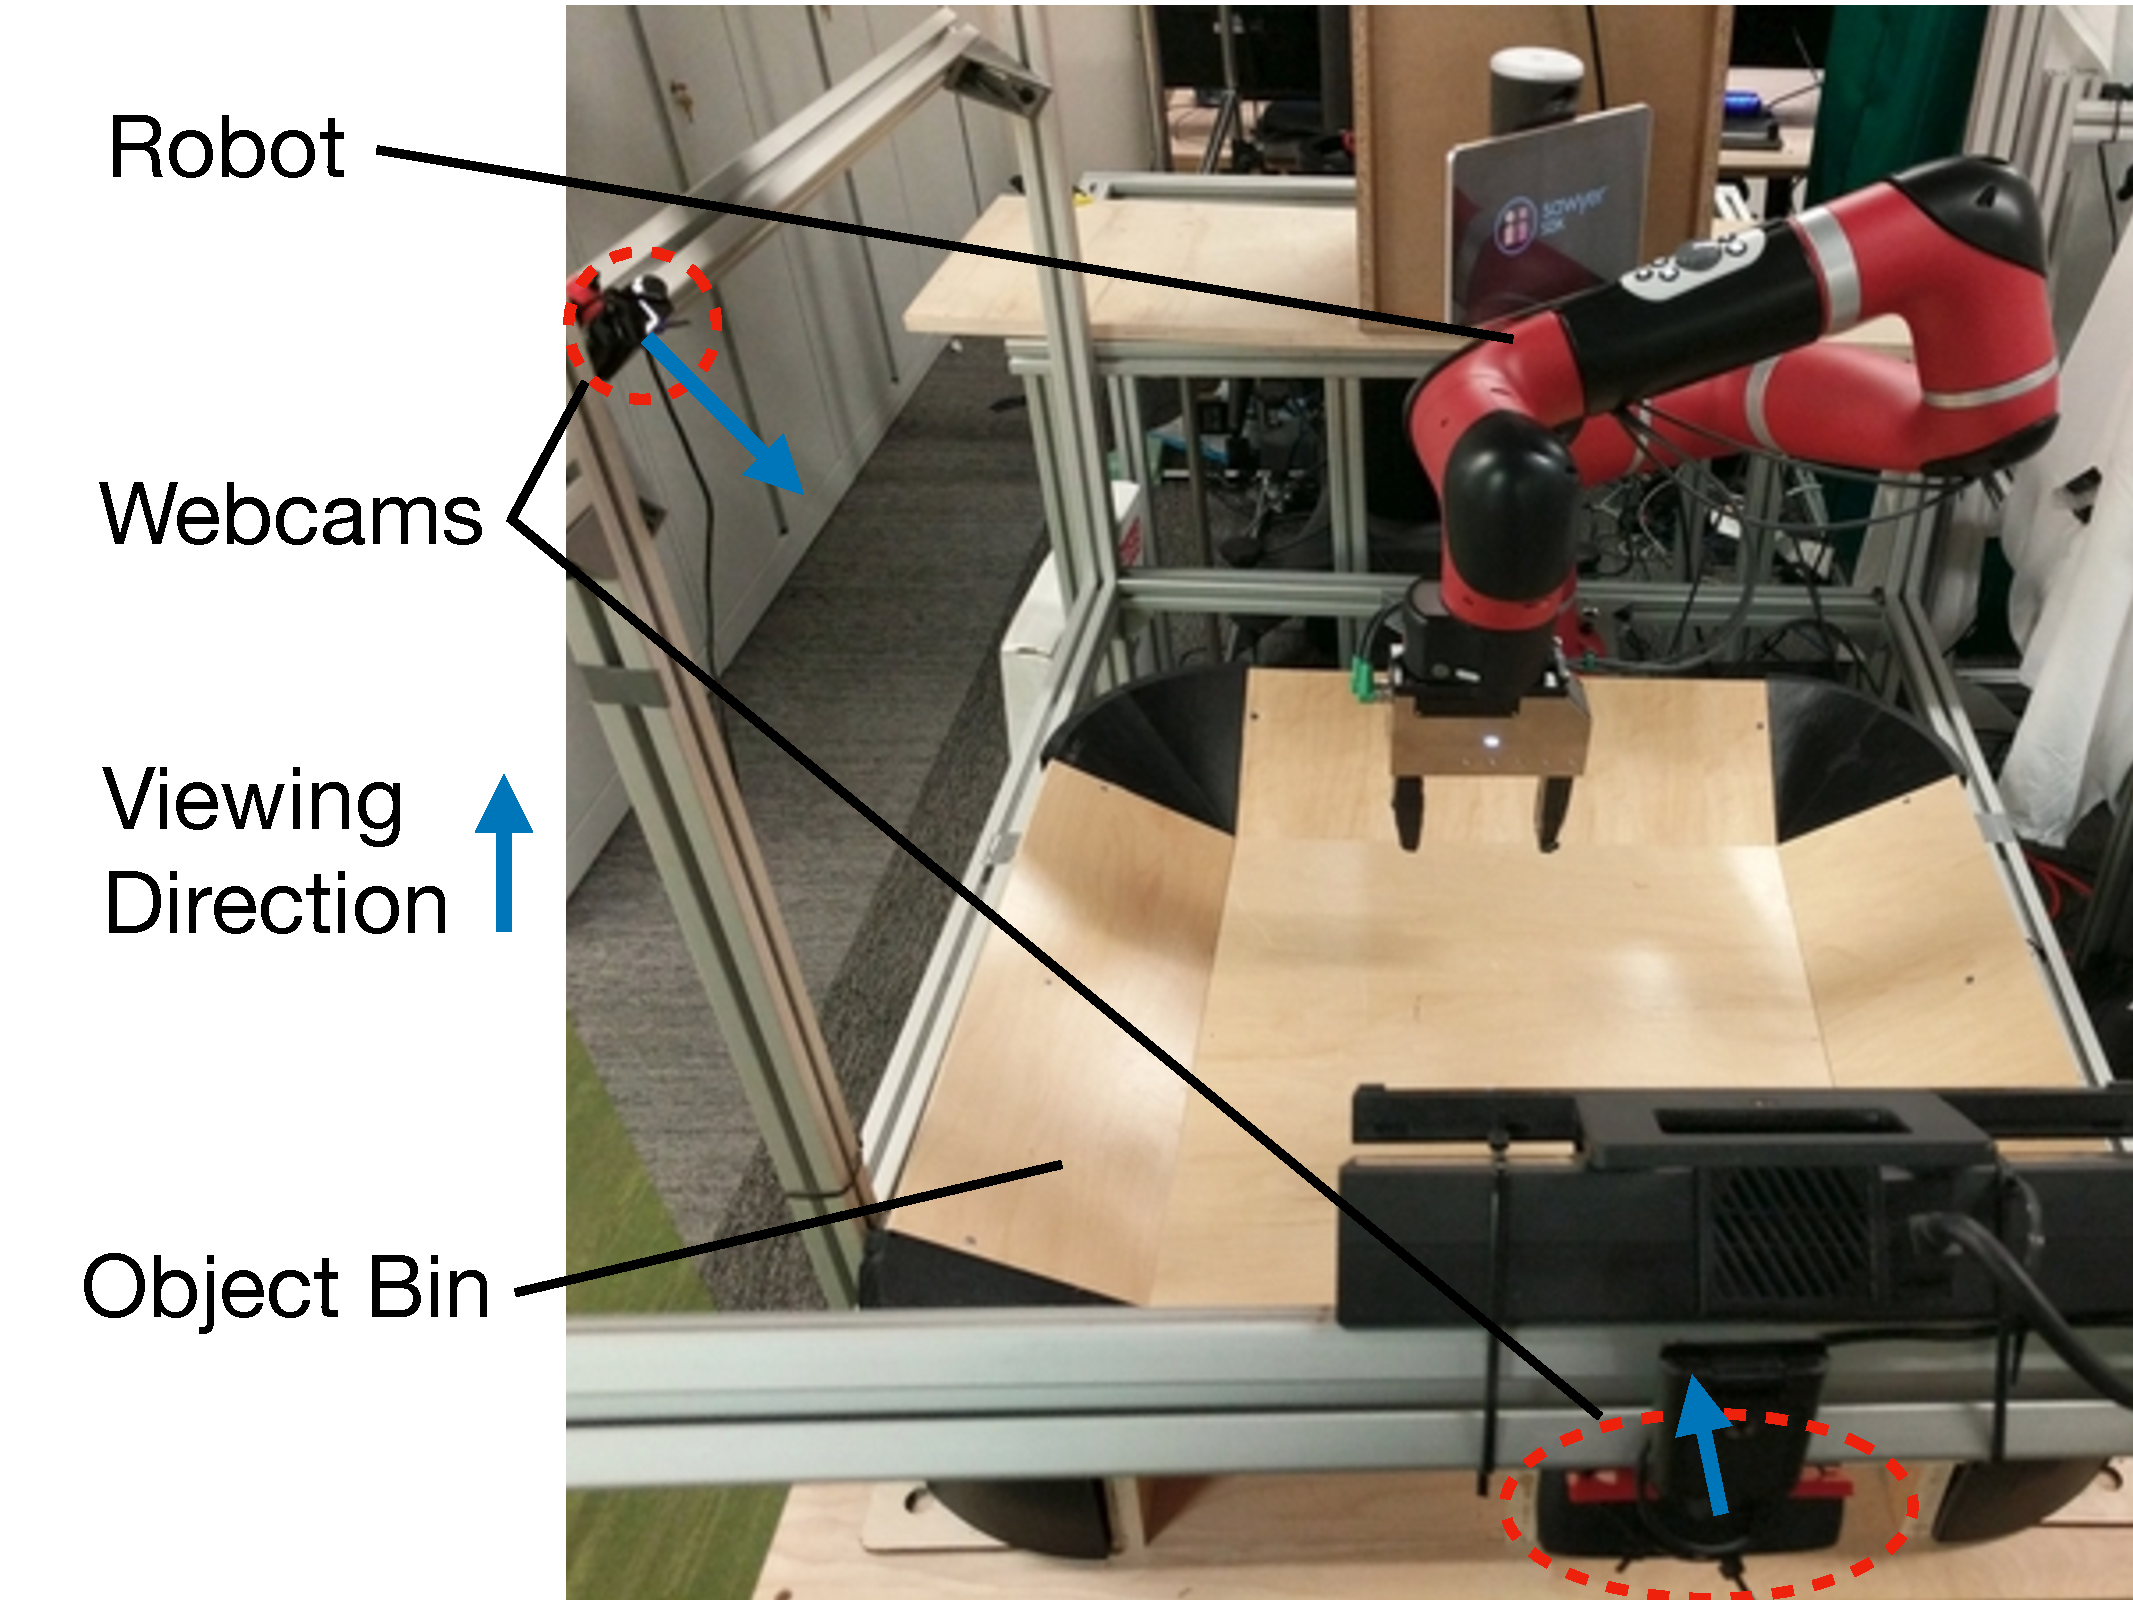
\includegraphics[width=0.45\columnwidth]{images_general/robot_setup_scheme.pdf}
	\caption{\small{Robot setup, with 2 standard web-cams arranged at different viewing angles.}}	\label{fig:robot_setup}
\end{wrapfigure}
\label{sec:experiments}
In this section we present both qualitative and quantitative  performance evaluations of visual MPC on various manipulation tasks assessing the degree of generalization and comparing different prediction models and cost functions and with a hand-crafted baseline.

\noindent \textbf{Qualitative Evaluation}
In figures \ref{fig:example_traj} and \ref{fig:tile_2} we present a set of qualitative experiments showing that visual MPC trained fully self-supervised is capable of solving a wide range of complex tasks.
%\begin{enumerate}
%	\item Multiple-object relocation tasks through pushing
%	\item Combined obstacle avoidance and object relocation tasks in the presence of occlusion
%	\item Object relocation through combined pushing and grasping
%	\item Object relocation task with external perturbations of the object position
%	\item Relative object rearrangment tasks, including multiple object rearrangement
%	\item Handling of deformable objects, such as towel folding and cloth folding
%\end{enumerate}
Videos for the qualitative examples are at the following webpage\footnote{https://sites.google.com/view/visualforesight/}

\noindent \textbf{Quantitative Evaluation} In order to perform quantitative comparisons, we define a set of benchmark tasks where the robot is required to move object(s) into a goal configuration. For measuring success, we use a distance-based evaluation where a human annotates the positions of the objects after pushing allowing us to compute the remaining distance to the goal.
%\begin{enumerate}
%	\item [\ref{subsec:sna_experiments}] How important is the model's ability to handle occlusion? How do temporal skip-connections introduced in the SNA-model affect performance compared to the DNA model without skip-connections?
%	\item [\ref{susbsec:reg_cost_exp}] How important is the system's ability to update the belief of \emph{where} the object is? How is performance affected by using a registration-based cost function, and how does closed-loop visual MPC compare to closed-loop visual MPC and visual MPC with off-the-shelf tracking?
%	\item [\ref{subsec:eval_classifier}] How does visual MPC with a classifier-based cost function compare to visual MPC with pixel MSE-based cost function on relative object rearrangement tasks?
%	\item [\ref{subsec:multi_task_bench}] How does visual MPC compare to a hand-engineered controller that relies on a calibrated camera on a large set of diverse tasks?
%\end{enumerate}

\subsection{Comparing Video Prediction Architectures}
\label{subsec:sna_experiments}
We first aim to answer the question: Does  visual MPC using the occlusion-aware SNA video prediction model that includes temporal skip connections outperform visual MPC with the dynamic neural advection model (DNA)\cite{foresight} \emph{without} temporal skip-connections?
We evaluate on multi-objective tasks where one object must be pushed without disturbing another.

	%%SL.10.16: This sounds really disappointing. Presumably we do lots of other cool stuff too? What about classifier, towels, rearrangement and placing tasks?
	
	%%SL.10.16: do we use the same test procedure in other subsections too? If so, let's have a separate subsection to describe the experiment, and then separate subsections for results, otherwise there will be a lot of duplication. Don't just staple the experiment sections from different papers together...
	%\todo{\autoref{fig:long_distance_task} shows an example task for the pushing benchmark.}
	%%SL.10.16: I think these "bare bones" pictures with no distractors are really boring. Can we mostly show interesting tasks with lots of distractors, and contain the simple pushing tasks in one subsection? If we have lots of pictures of the simple tasks, people will conclude that the method only works with one object in the scene.
	%We collected 20 trajectories with 3 novel objects and 1 training object. \autoref{table:res_dna_sna} shows the results for the pushing benchmark. The column \textit{distance} refers to the mean distance between the goal pixel and the designated pixel at the final time-step. The column \textit{improvement} indicates how much the designated pixel of the objects was moved closer to their goal (or further away for negative values) compared to the starting location. The true locations of the designated pixels after pushing were annotated by a human labeler.
	
	%The results in \autoref{table:res_dna_sna} show that our proposed planning cost in \autoref{eq:cost}
	%%SL.10.16: wait, what? I thought this section was evaluating models, not costs? Can we separate these out, first evaluate models, then costs, to reflect the organization in the paper?
	%substantially outperforms the planning cost used in prior work~\cite{foresight}. The performance of the SNA model in these experiments is comparable to the DNA model~\cite{foresight} when both use the expected-distance planning cost, since this task does not involve any occlusions.
	%%SL.10.16: Hmm... OK, perhaps if we're going to evaluate costs and models simultaneously like this, we need to organize the sections more clearly. Maybe it would really help in that case to separate out experiment setup (how the methods care compared) from the results (how they stack up). And for each section, ask yourself: what is the question these experiments are trying to answer? It should be obvious from the writing. Right now, I feel like the experiments section looks too much like experiments sections from different papers stapled together. They need to more integrated and focused on achieving the paper's aims: state the research questions, and explain how each experiment subsection answers one or more of those questions



\begin{table}
\centering
{\footnotesize
\begin{tabular}{lcc}
	\toprule
         &  \thead{moved imp. \\ $\pm$ std err. of mean} &   \thead{stationary imp. \\ $\pm$ std err. of mean}  \\
         \midrule
  DNA \cite{foresight} & 0.83 $\pm$0.25 &  -1.1 $\pm$ 0.2\\ 
  SNA & \textbf{10.6 $\pm$ 0.82} & \textbf{-1.5 $\pm$ 0.2} \\
  \bottomrule
\end{tabular}
}
\caption{Results for multi-objective pushing on 8 object/goal configurations with 2 seen and 2 novel objects. Values indicate improvement in distance from starting position, higher is better. Units are pixels in the 64x64 images.} 
\label{table:mult_obj}
\end{table}

To examine whether our skip-connection model (SNA) helps with handling occlusions, we devised a task that requires the robot to push one object, while keeping another object stationary. When the stationary object is in the way, the robot must move the target object around it. This is illustrated on the left side of \autoref{fig:goingaroundocclusion} in the appendix. While pushing the target object, the gripper may occlude the stationary object, and the task can only be performed successfully if the model can make accurate predictions through this occlusion. These tasks are specified by selecting one starting pixel on the target object, one goal pixel location for the target object, and one pixel location on the obstacle used both as the start and the goal to indicate that it should not be moved. %The obstacle is commanded to remain stationary, by choosing the target position to be at the same location as the initial position. For the target object the destination is chosen on the other side of the obstacle.

We use four different object arrangements with two training objects and two objects that were not seen during training. We find that, in most cases, the SNA model is able to find a valid trajectory, while the DNA model, that is not able to handle occlusion, is mostly unable to find a solution. The results of our quantitative comparisons are shown in \autoref{table:mult_obj}, indicating that temporal skip-connections indeed help with handling occlusion in combined pushing and obstacle avoidance tasks. 
%%SL.10.16: It would help if the experimental conclusion at the end of this section is an answer to  question posed earlier in the experiments. I also think it makes too big of a deal out of the SNA thing -- this is not the SNA paper, we don't need to push on this so hard!

\subsection{Evaluating Registration-based Cost Functions}
\label{susbsec:reg_cost_exp}
%%SL.10.16: This is very misleading, all of the experiments are closed-loop!

\begin{table}
	{\footnotesize
		\begin{center}
			\begin{tabular}{lcc}
				\toprule
				%				 & \multicolumn{2}{c}{fraction of successful runs} \\
				& Short & Long \\
				\midrule
				Visual MPC $+$ predictor propagation  & 83\% & 20\% \\
				Visual MPC $+$ OpenCV tracking  & 83\%  & 45\% \\
				Visual MPC $+$ registration network & 83\% & \textbf{66\%}  \\
				\bottomrule
			\end{tabular}
		\end{center}
	}
	\caption{\small Success rate for long-distance pushing benchmark with 20 different object/goal configurations and short-distance benchmark with 15 object/goal configurations. Success is defined as bringing the object closer than 15 pixels to the goal, which corresponds to around $7.5cm$.}
	\label{table:res_long_short}
\end{table}
In this section we ask: How important  is it to update the model's belief of where the target objects currently are? 
We first provide two qualitative examples:

In example (1) of figure \ref{fig:example_traj} the task is to bring the stuffed animal to a particular location in 3D-space on the other side of the arena. To test the system's reaction to perturbations that could be encountered in open-world settings, during execution a human knocks the object out of the robot's hand. The experiment shows that visual MPC is able to naturally perform a new grasp attempt and bring the object to the goal.

In figure \ref{fig:push_retry} in the appendix, the task is to push the bottle to point marked with the green dot. In this the system recovers from an initial failure.

The next question we investigate is: How much does this matter for short horizon versus long horizon tasks? 
In this experiment, we disable the gripper control, which requires the robot to push objects to the target. We compare two variants of updating the positions of the designated pixel when using a pixel-distance based cost function. The first is a cost function that uses a registration-based method, trained in a fully self-supervised fashion, and the second is with a cost function that uses off-the shelf tracking from OpenCV \cite{babenko2009visual}. Additionally we compare to visual MPC that uses the video-prediction model's own prior predictions to update the current position of the designated pixel, rather than tracking the object with registration or tracking.

%SL.10.16: Before talking about videos, explain what this experiment section is actually studying! What is the question? What are you evaluating? Why?

%%SL.10.16: again, not entirely clear what question this is trying to answer

%\begin{figure}
%	\centering
%	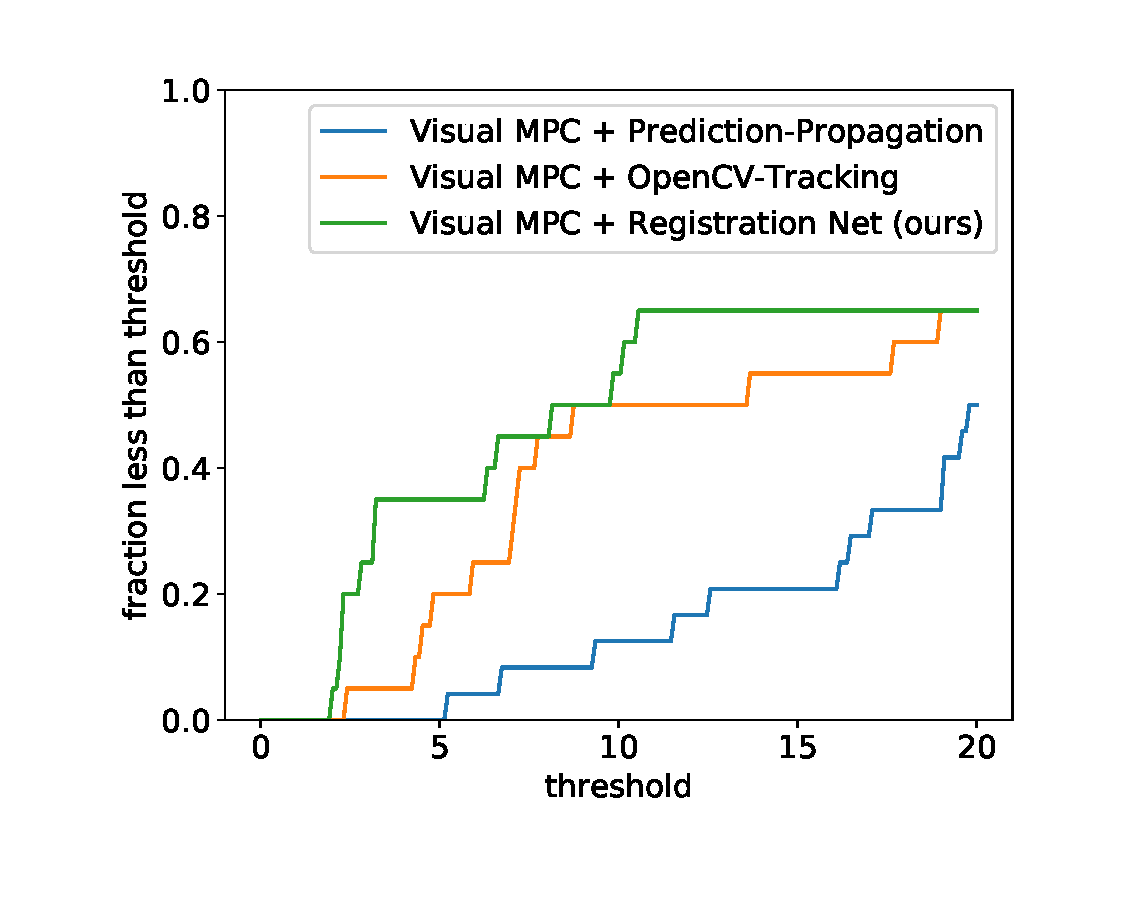
\includegraphics[width=0.8\columnwidth]{images_rfr/pushlong_bench_same_range.pdf}
%	\caption{\small{Results for long pushing tasks with 20 objects not seen during training, showing fraction of runs where final distance is lower than threshold. Our method shows a clear gains over OpenCV tracking and predictor propagation.}}
%	\label{fig:push_bench_long}
%\end{figure}

We evaluate our method on 20 long-distance and 15 short-distance pushing tasks. For long distance tasks the initial distance between the object and its goal-position is $30cm$ while for short distance tasks it is $15cm$. Table \ref{table:res_long_short} lists quantitative comparisons showing that on the long distance benchmark visual MPC using the registration-based cost not only outperforms prior work \cite{sna}, but also outperforms the hand-designed, supervised object tracker \cite{babenko2009visual}. By contrast for the short distance benchmark, all methods perform comparably. Thus, theses results demonstrate the importance of closed loop control for \emph{long-horizon tasks}, while for short-horizon tasks object tracking appears to be irrelevant. 

\subsection{Evaluating Classifier-based Cost Function}
\label{subsec:eval_classifier}

\begin{figure}
	\centering
	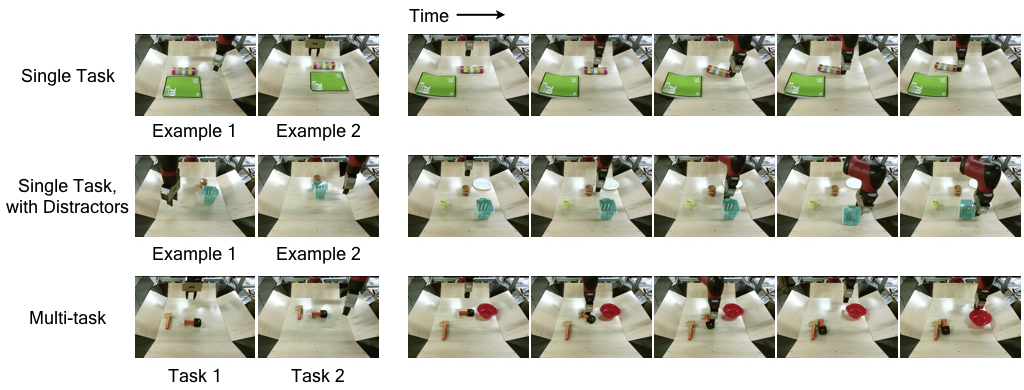
\includegraphics[width=1.0\columnwidth]{images_cls/cls_results.jpeg}
	\caption{\small Object arrangement performance of our goal classifier with distractor objects and with two tasks. The left shows a subset of the 5 positive examples that are provided for inferring the goal classifier(s), while the right shows the robot executing the specified task(s) via visual planning.}
	\label{fig:cls_results}
	\vspace{-0.3cm}
\end{figure}

% Here we study the question: How does the success rate of visual MPC using the proposed classifier-based cost function compare to a baseline based on pixel-distance and DSAE in a relative object arrangement task?

The goal of the classifier-based cost function is to provide an easy way to compute an objective for new tasks from a few observations of success for that task, so we compare our approach to alternative and prior methods for doing so under the same assumptions: pixel distance and latent space distance. In the latter, we measure the distance between the current and goal observations in a learned latent space, obtained by training an autoencoder (DSAE) \cite{dsae} on the same data used for our classifier. Because we are considering a different form of task specification, we do not compare the classifier-based cost function to costs based on user-designated pixels or registration.

%We evaluate our learned classifier on the predictions made by the video prediction model \todo{unclear, how exactly do you evaluate the classifier?} and derive the cost used for planning from the predicted probability of success. 

To collect data for meta-training the classifier, we randomly select a pair of objects from our set of training objects, and position them into many different relative positions, recording the image for each configuration. One task corresponds to a particular relative positioning of two objects, e.g. the first object to the left of the second, and we construct positive and negative examples for this task by labeling the aforementioned images. We randomly position the arm in each image, as it is not a determiner of task success. A good objective should ignore the position of the arm. We also include randomly-positioned distractor objects in about a third of the collected images.

We evaluate the classifier-based cost function in three different experimental settings. In the first setting, the goal is to arrange two objects into a specified relative arrangement. The second setting is the same, but with distractor objects present. In the final, most challenging setting, the goal is to achieve two tasks in sequence. We provide positive examples for both tasks, infer the classifier for both task, perform MPC for the first task until completion, followed by MPC for the second task. To evaluate the ability to generalize to new goals and settings, we use novel, held-out objects for all of the task and distractor objects in our evaluation. 

We qualitatively visualize the benchmark tasks in Figure~\ref{fig:cls_results}.
On the left, we show a subset of the five images provided to illustrate the task(s), and on the left, we show the motions performed by the robot. We see that the robot is able to execute motions which lead to a correct relative positioning of the objects.

We quantitatively evaluate each method across 20 tasks, including $10$ unique object pairs. The results, shown in Figure~\ref{fig:cls_charts}, indicate that the distance-based metrics
%%SL.10.16: you mean the method *in this paper*?
struggle to infer the goal of the task, while our approach leads to substantially more successful behavior on average.
\todo{explain how exactly you measure success} 
%%SL.10.16: what is the conclusion from all this? how do the different methods of specifying costs stack up?

%%SL.10.16: where are qualitative results and discussion of cloth?


\begin{figure}
    \centering
    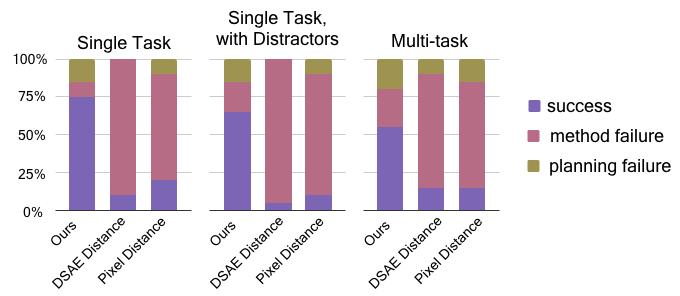
\includegraphics[width=0.48\textwidth]{images_cls/cls_charts.jpeg}
    \caption{\small Quantitative performance of visual planning for object rearrangement tasks across different goal specification methods: our meta-learned classifier, DSAE~\cite{dsae}, and pixel error. Where possible, we include break down the cause of failures into errors caused by inaccurate prediction or planning and those caused by an inaccurate goal classifier.}
    \label{fig:cls_charts}
    \vspace{-0.3cm}
\end{figure}


\subsection{Evaluating Multi-Task Performance}
\label{subsec:multi_task_bench}
One of the key motivations for visual MPC is to build a system that can solve a \emph{wide variety} of different tasks, involving completely different objects, physics and semantics. Examples for tasks that can be solved with visual MPC are shown in figure \ref{fig:example_traj} and \ref{fig:tile_2}. The tasks (1) and (2) are object rearrangement tasks, in task (3) a towel needs to be wrapped around an object while keeping the object stationary. The example shown in (4) and all examples in figure \ref{fig:cls_results} show relative object rearrangement tasks. Examples (5) and (6) show the same "placing task" where an object needs to be grasped and placed onto a plate. In (7) the task is to move the black object to the goal location while avoiding the obstacle in the middle which is marked with a designated- and goal-pixel.

The generality of visual MPC mainly stems from two components --- the generality of the visual dynamics model and the generality of the task definition.
We found that the dynamics model often generalizes well to objects outside of the training set, if they have similar properties to the objects it was trained with. For example, trajectory (4) in figure \ref{fig:tile_2} shows the model predicting a pair of shorts being folded, although the model never encountered shorts during training, towels and shirts were the only cloths that were part of the training set. It is worth noting that, in all qualitative examples, the predictions are performed by the same model for objects not part of the training set.
The second component allowing for generality is the high degree of flexibility for task definition. Using designated pixels object positioning tasks can be defined in 3D space, as shown examples (1) and (2) in figure and examples (3)-(5) in figure \ref{fig:tile_2}, when adding a goal-image the positioning accuracy can be improved as thanks to the presented registration scheme. For tasks where we care about \emph{relative} rather than absolute positioning a meta-learned classifier can be used.

Next we present a benchmark to quantitatively answer the following question: How does visual MPC compare to a hand-engineered baseline on a large number of diverse tasks?  

\noindent \textbf{Hand-crafted Baseline} For this comparison we engineered a simple trajectory generator to perform a grasp at the location of the initial designated pixel, lift the arm and bring it to the position of the goal-pixel. A camera calibration was performed to carry out the necessary conversions between image-space and robot work-space coordinates. For simplicity, the baseline controller executes open-loop. Therefore to allow for a fair comparison visual-MPC is also executed open-loop, i.e. no registration or tracking is used.

Altogether we selected 16 tasks, some of them being identical to the qualitative examples presented earlier.
The results of the benchmark, shown in table \ref{table:cloth_folding}, indicate that visual MPC clearly outperforms the baseline. 
Visual MPC succeeded for most of the benchmark tasks. While the baseline succeeded for some of the cloth folding tasks, but failed for almost all of the object relocation tasks. We attribute this to the fact that it does not reason about physics, therefore it is lacking the capability of positioning the end-effector in a location that is appropriate for grasping or pushing. 

\begin{figure}
	\centering
	\includegraphics[width=1\columnwidth]{images_general/tile_2.png}
	\caption{Visual MPC successfully solves a wide variety of tasks including multi-objective tasks, such as placing an object on a plate (row 5 and 6), object positioning with obstacle avoidance (row 7) and folding shorts (row 8).   
		\label{fig:tile_2}}
\end{figure}

\label{subsec:cloth_folding_data}
\begin{table}
\centering
{\footnotesize
\begin{tabular}{lcc}
	\toprule
         &  \thead{\% of Trials with \\ Final Pixel Distance $< 15$}   \\
         \midrule
  Visual MPC & \textbf{75\%} \\ 
  Calibrated Camera Baseline & 18.75 \% \\
  \bottomrule
\end{tabular}
}
\caption{Results for a combined benchmark of 10 hard object pushing and grasping tasks, along with 6 cloth folding tasks. Values indicate the percentage of trials which ended with the object closer than a threshold distance (measured in pixels) to the designated goal. Higher is better.} 
\label{table:cloth_folding}
\end{table}

\noindent \textbf{Discussion}
Generalization and multi-task performance is arguably one of the biggest challenges in robotic manipulation today. While deep learning has relieved us from much of the problem-specific engineering, most of the works either require extensive amounts of labeled data or in the case of deep reinforcement learning, focus on the mastery of single tasks while relying on human-provided reward signals. 
From the experiments with visual MPC, especially the qualitative examples and the multi-task benchmark, we can conclude that visual MPC \emph{generalizes} to a wide range of tasks it has never seen during training. This is in contrast to many model-free approaches for robotic control which often struggle to perform well on novel tasks. Most of the generalization performance is likely a result of large-scale self-supervised learning, which allows to acquire a rich dynamics model of the environment. 
% pushing benchmark with and without tracking
% grasping
% experiments with stochastic models, optimistic/pessimistic planning



\section{Conclusion}
We presented an algorithm that leverages self-supervision from visual prediction to learn a deep dynamics model on images, and show how it can be embedded into a  planning framework to solve a variety of robotic control tasks. We demonstrate that visual model-predictive control is able to successfully perform multi-object manipulation, pushing, picking and placing, and cloth-folding tasks -- all within a single framework. These tasks involve complex contact dynamics as well as deformable objects, indicating that the same sensory prediction model can be used to capture a wide variety of environment dynamics with enough accuracy to allow for control.

%%SL.10.16: I think the discussion below is not quite a good fit for future work. It's important to understand what the *purpose* of the future work section is. Contrary to what the name might imply, the purpose of future work is *not* to actually discuss future work. The purpose of future work is to inspire the reader that your work has lots of potential to lead to new and exciting research. You should *not* usually talk about immediate next steps you plan to take, but rather all the awesome stuff *enabled* by your work.

%%SL.10.16: What I would recommend is to have one paragraph on limitations (which is actually future work in disguise), and then a future work paragraph meant to inspire the reader about all the great stuff you could do with this method, ending on a very high note in the end about the generality of entirely self-supervised robotic deep model-based RL algorithms.

\noindent \textbf{Limitations}
The main limitations of the presented framework are that all target objects need to be visible throughout execution, it is currently not possible to handle partially observed domains. This is especially important for tasks that require objects to be brought into occlusion (or taken out of occlusion), for example putting an object in a box and closing it. Another limitation is that the tasks are still of only medium duration and usually only touch one or two objects. Longer-term planning remains an open problem. Lastly, the fidelity of object positioning is still significantly below what humans can achieve.

\noindent \textbf{Possible future directions}
The key advantage of a model-based deep-reinforcement learning algorithm like visual MPC is that it \emph{generalizes} to tasks it has never encountered before. This makes visual MPC a good candidate for a building block of future robotic manipulation systems that will be able solve an even wider range of complex tasks with much longer horizons. 


% use section* for acknowledgment
\ifCLASSOPTIONcompsoc
  % The Computer Society usually uses the plural form
%  \section*{Acknowledgments}
\else
  % regular IEEE prefers the singular form
%  \section*{Acknowledgment}
\fi


%The authors would like to thank...The authors would like to thank...The authors would like to thank...The authors would like to thank...The authors would like to thank...The authors would like to thank...The authors would like to thank...The authors would like to thank...The authors would like to thank...The authors would like to thank...


% Can use something like this to put references on a page
% by themselves when using endfloat and the captionsoff option.
\ifCLASSOPTIONcaptionsoff
  \newpage
\fi



% trigger a \newpage just before the given reference
% number - used to balance the columns on the last page
% adjust value as needed - may need to be readjusted if
% the document is modified later
%\IEEEtriggeratref{8}
% The "triggered" command can be changed if desired:
%\IEEEtriggercmd{\enlargethispage{-5in}}

% references section

% can use a bibliography generated by BibTeX as a .bbl file
% BibTeX documentation can be easily obtained at:
% http://mirror.ctan.org/biblio/bibtex/contrib/doc/
% The IEEEtran BibTeX style support page is at:
% http://www.michaelshell.org/tex/ieeetran/bibtex/
%\bibliographystyle{IEEEtran}
% argument is your BibTeX string definitions and bibliography database(s)
%\bibliography{IEEEabrv,../bib/paper}
%
% <OR> manually copy in the resultant .bbl file
% set second argument of \begin to the number of references
% (used to reserve space for the reference number labels box)
% \begin{thebibliography}{1}

% \bibitem{IEEEhowto:kopka}
% H.~Kopka and P.~W. Daly, \emph{A Guide to \LaTeX}, 3rd~ed.\hskip 1em plus
%   0.5em minus 0.4em\relax Harlow, England: Addison-Wesley, 1999.

% \end{thebibliography}

\bibliographystyle{IEEEtran}
\bibliography{mybib}
% biography section
% 
% If you have an EPS/PDF photo (graphicx package needed) extra braces are
% needed around the contents of the optional argument to biography to prevent
% the LaTeX parser from getting confused when it sees the complicated
% \includegraphics command within an optional argument. (You could create
% your own custom macro containing the \includegraphics command to make things
% simpler here.)
%\begin{IEEEbiography}[{\includegraphics[width=1in,height=1.25in,clip,keepaspectratio]{mshell}}]{Michael Shell}
% or if you just want to reserve a space for a photo:
\vskip -13mm

\begin{IEEEbiographynophoto}{Frederik Ebert}
Frederik Ebert received a BS in Mechatronics and Information Technology as well a MS in "Robotics, Cognition, Intelligence (RCI)" from the Technical University of Munich (TUM). He is currently a PhD student at Berkeley Artifical Intelligence Research (BAIR). % institute where he focuses on developing algorithms for robotic manipulation combining ideas from computer vision, machine learning and control.
\end{IEEEbiographynophoto}
\vskip -13mm

% if you will not have a photo at all:
\begin{IEEEbiographynophoto}{Chelsea Finn}
Chelsea Finn is currently a research scientist at Google Brain and a post-doctoral scholar at UC Berkeley. %, and will join the Computer Science faculty at Stanford in 2019. %Her research focuses on algorithms that can enable agents to autonomously learn a range of complex skills. 
She received a BS in Electrical Engineering and Computer Science from MIT and a PhD in Computer Science from UC Berkeley.
\end{IEEEbiographynophoto}
\vskip -13mm

% insert where needed to balance the two columns on the last page with
% biographies
%\newpage

\begin{IEEEbiographynophoto}{Annie Xie}
% Biography text here.
Annie Xie is pursuing a B.S. degree in Electrical Engineering and Computer Science at UC Berkeley. %Her research interests are in the areas of computer vision and robot learning.
\end{IEEEbiographynophoto}
\vskip -13mm

\begin{IEEEbiographynophoto}{Sudeep Dasari}
	Sudeep Dasari is a 4th year student at UC Berkeley pursuing a B.S in Electrical Engineering and Computer Science. %His primary research interests are computer vision, machine learning, and robotic control.
\end{IEEEbiographynophoto}
\vskip -13mm

\begin{IEEEbiographynophoto}{Alex Lee}
	Alex Lee received a BS in Electrical Engineering and Computer Science from UC Berkeley and is currently pursuing a PhD in Computer Science from UC Berkeley. %His work focuses on algorithms that can enable robots to learn complex sensorimotor skills.
\end{IEEEbiographynophoto}
\vskip -13mm

\begin{IEEEbiographynophoto}{Sergey Levine}
Sergey Levine received a BS and MS in Computer Science from Stanford, and a Ph.D. in Computer Science from Stanford. He is currently on the faculty of the Department of Electrical Engineering and Computer Sciences at UC Berkeley. %His work focuses on machine learning for decision making and control, with an emphasis on deep learning and reinforcement learning algorithms.
\end{IEEEbiographynophoto}

% You can push biographies down or up by placing
% a \vfill before or after them. The appropriate
% use of \vfill depends on what kind of text is
% on the last page and whether or not the columns
% are being equalized.

%\vfill

% Can be used to pull up biographies so that the bottom of the last one
% is flush with the other column.
%\enlargethispage{-5in}

\appendices
\newpage

\section{Skip Connection Neural Advection Model}
\label{sec:skipcon}

Our video prediction model, shown in ~\autoref{fig:prediction_model}, is inspired by the dynamic neural advection (DNA) model proposed by~\cite{finn_nips} and it is a variant of the SNA model proposed by~\cite{sna}. The model uses a convolutional LSTM~\cite{convlstm} to predict future frames. The prediction is initialized with an initial sequence of 2 ground truth frames, and predicts 13 futures frames. The model predicts these frames by iteratively making next-frame predictions and feeding those predictions back to itself. Each predicted frame, is given by a compositing layer, which composes intermediate frames with predicted compositing masks. The intermediate frames include the previous 2 frames and transformed versions them. To easily allow various transformations for different parts of the image, we predict 8 transformed frames, 4 of which are transformed from the previous frame, and the other 4 from the frame 2 steps in the past. These intermediate frames are then combined with compositing masks, which are also predicted by the convolutional LSTM. For simplicity, we collectively refer to these transformations as a single transformation $\hat{F}_{t+1 \leftarrow t}$ in~\autoref{simple_dna}. In addition, the first frame of the sequence is also given as one of the intermediate frames~\cite{sna}.

To enable action conditioning, the robot action at each time step is passed to all the convolutional layers of the main network, by concatenating it along the channel dimension of the inputs of these layers. Since they are vectors with no spatial dimensions, they are replicated spatially to match the spatial dimensions of the inputs.

The SNA variant that we use incorporate the architectural improvements proposed by~\cite{savp}. Each convolutional layer is followed by instance normalization \cite{instancenorm} and ReLU activations. We also use instance normalization on the LSTM pre-activations (i.e., the input, forget, and output gates, as well as the transformed and next cell of the LSTM). In addition, we modify the spatial downsampling and upsampling mechanisms. Standard subsampling and upsampling between convolutions is known to produce artifacts for dense image generation tasks~\cite{odena2016deconvolution,Niklaus_ICCV_2017}. In the encoding layers, we reduce the spatial resolution of the feature maps by average pooling, and in the decoding layers, we increase the resolution by using bilinear interpolation. All convolutions in the generator use a stride of 1. The actions are concatenated to the inputs of all the convolutional layers of the main network, as opposed to only the bottleneck.

\begin{wrapfigure}{r}{.37\columnwidth}
	\centering
	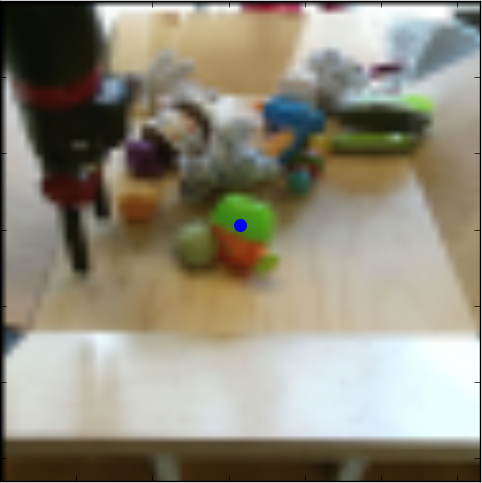
\includegraphics[width=0.37\columnwidth]{images_sna/occlusionaware/img_desigpixb0.png}
	\caption{The blue dot indicates the designated pixel}
	\label{fig:desig_pix_bluedot}
\end{wrapfigure}

We provide an example of the skip connection neural advection (SNA) model recovering from occlusion in \autoref{fig:pix_reappear}. In this figure, the arm is predicted to move in front of the designated pixel, marked in blue in \autoref{fig:desig_pix_bluedot}. The predictions of the DNA model, shown in figure \autoref{fig:pix_reappear}(b), contain incorrect motion of the marked object, as shown in the heatmaps visualizing $\hat{P}_t$, although the arm actually passes in front of it. This is because the DNA model cannot recover information about an object that it has `overwritten' during its predictions, causing the model to predict that the pixel \emph{moves with the arm}. We identified this as one of the major causes of planning failure using the DNA model. By contrast our SNA model predicts that the occluded object will not move, shown in figure  \autoref{fig:pix_reappear}(a).

\begin{figure}
	\centering
	\begin{subfigure}{0.9\columnwidth}
		\centering
		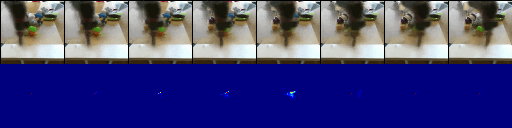
\includegraphics[width=1.\linewidth]{images_sna/occlusionaware/cdna_1ststep_bckgd_gen_pixb0_overtime.png}
		\caption{Skip connection neural advection (SNA) does not erase or move objects in the background}
		\label{fig:Ng1}
	\end{subfigure}
	\begin{subfigure}{0.9\columnwidth}
		\centering
		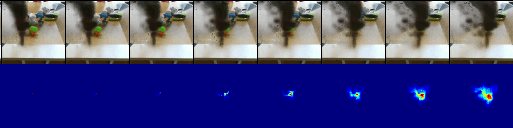
\includegraphics[width=1.0\linewidth]{images_sna/occlusionaware/orig_dna_gen_pixb0_overtime.png}
		\caption{Standard DNA \cite{foresight} exhibits undesirable movement of the distribution $P_{d}(t)$ and erases the background}
	\end{subfigure}
	\caption{
		%\protect\subref{fig:Ng1} 
		Top rows: Predicted images of arm moving \textit{in front of} green object with designated pixel (as indicated in \autoref{fig:desig_pix_bluedot}). 
		%(\protect\subref{fig:Ng2}) 
		Bottom rows: Predicted probability distributions $P_{d}(t)$ of designated pixel obtained by repeatedly applying transformations.}
	\label{fig:pix_reappear}
\end{figure}

\section{Improved Action Sampling Distributions for Data Collection}
\label{sec:folding_sampling}
In order to collect meaningful interaction data for learning folding of deformable objects such as towels and cloth, we found that the grasping primitive can be slightly adapted to increase the likelihood of encountering states where cloths are actually folded. When using actions sampled from a simple distribution or the previously-described distribution, clothing would become tangled up. To improve the efficiency of folding cloths we use an action primitive similar to the grasping primitive, but additionally we reduce lateral motion of the end-effector when the gripper is close to the table, thus reducing events where cloths become tangled up.

\section{Improvements of the CEM-Optimizer}
\label{sec:cem_improv}
In the model-predictive control setting, the action sequences found by the optimizer can be very different between execution real-world times steps. For example at one time step the optimizer might find a pushing action leading towards the goal and in the next time step it determines a grasping action to be optimal to reach the goal. Na\"{i}ve replanning at every time step can then result in alternating between a pushing and a grasping attempt indefinitely causing the agent to get stuck and not making any progress towards to goal. 

%%SL.10.15: It's not clear whether this is done in every experiment or just some experiments.
We can resolve this problem by modifying the sampling distribution of the first iteration of CEM so that the optimizer commits to the plan found in the previous time step. In the simplest version of CEM the sampling distribution at first iteration of CEM is chosen to be a Gaussian with diagonal covariance matrix and zero mean. We instead use the best action sequence found in the optimization of the \emph{previous} real-world time step as the mean for sampling new actions in the \emph{current} real-world time-step. Since this action sequence is optimized for the previous time step we only use the values $a_{2:T}$ and omit the first action. To sample actions close to the action sequence from the previous time step we reduce the entries of the diagonal covariance matrix for the first $T-1$ time steps. It is crucial that the last entry of the covariance matrix at the end of the horizon is not reduced otherwise no exploration could happen for the last time step causing poor performance at later time steps.

\section{Experimental Setup}
\label{sec:experiment_setup}
To train both our video-prediction and registration models, we collected 20,000 trajectories of pushing motions and 15,000 trajectories with gripper control, where the robot randomly picks and moves objects using the grasping reflex described in section \ref{sec:system}. The data collection process is fully autonomous, requiring human intervention only to change out the objects in front of the robot. The action space consisted of relative movements of the end-effector in cartesian space along the $x$, $y$, and $z$ axes, and for some parts of the dataset we also added azimuthal rotations of the gripper and a grasping action.

\section{Experimental Evaluation}

\begin{figure*}
    \centering    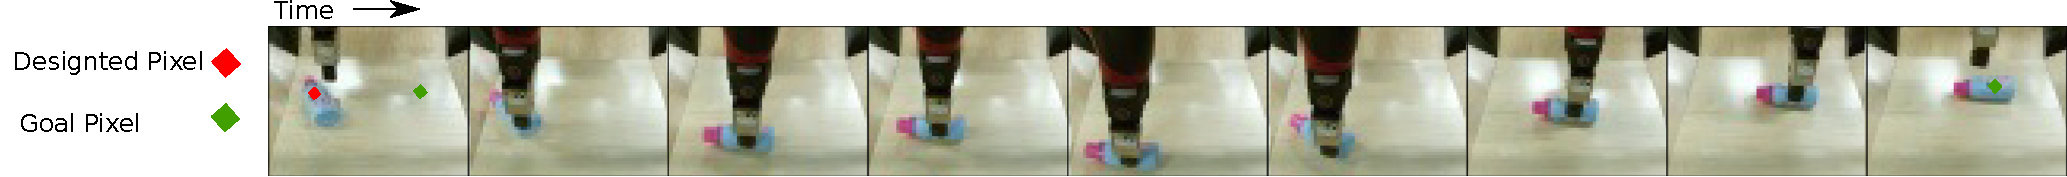
\includegraphics[width=1.0\textwidth]{images_rfr/push_correction.pdf}
    \caption{\small{Applying our method to a pushing task. In the first 3 time instants the object behaves unexpectedly, moving down. The tracking then allows the robot to retry, allowing it to eventually bring the object to the goal.}}
    \label{fig:push_retry}
\end{figure*}

\begin{figure*}
	\centering
	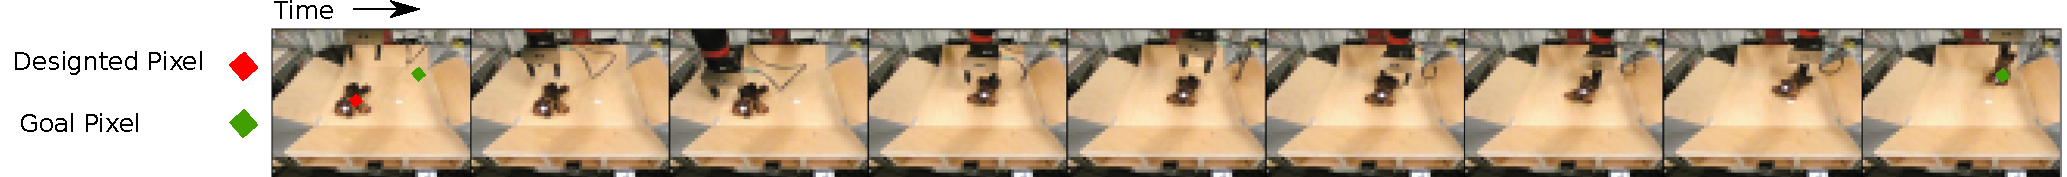
\includegraphics[width=1.0\textwidth]{images_rfr/pick_place_plush.pdf}
	\caption{\small{Retrying behavior of our method combining prehensile and non-prehensile manipulation. In the first 4 time instants shown the robot pushes the object. It then loses the object, and decides to grasp it pulling it all the way to the goal. Retrying is enabled by applying the learned registration to both camera views (here we only show the front view).}}
	\label{fig:push_grasp}
\end{figure*}

\subsection{Experiments with multiple-objects rearrangement with occlusion}

\autoref{fig:goingaroundocclusion} shows an example of the SNA model successfully predicting the position of the obstacle through an occlusion and finding a trajectory that avoids the obstacle. 

\begin{figure*}
	\centering
	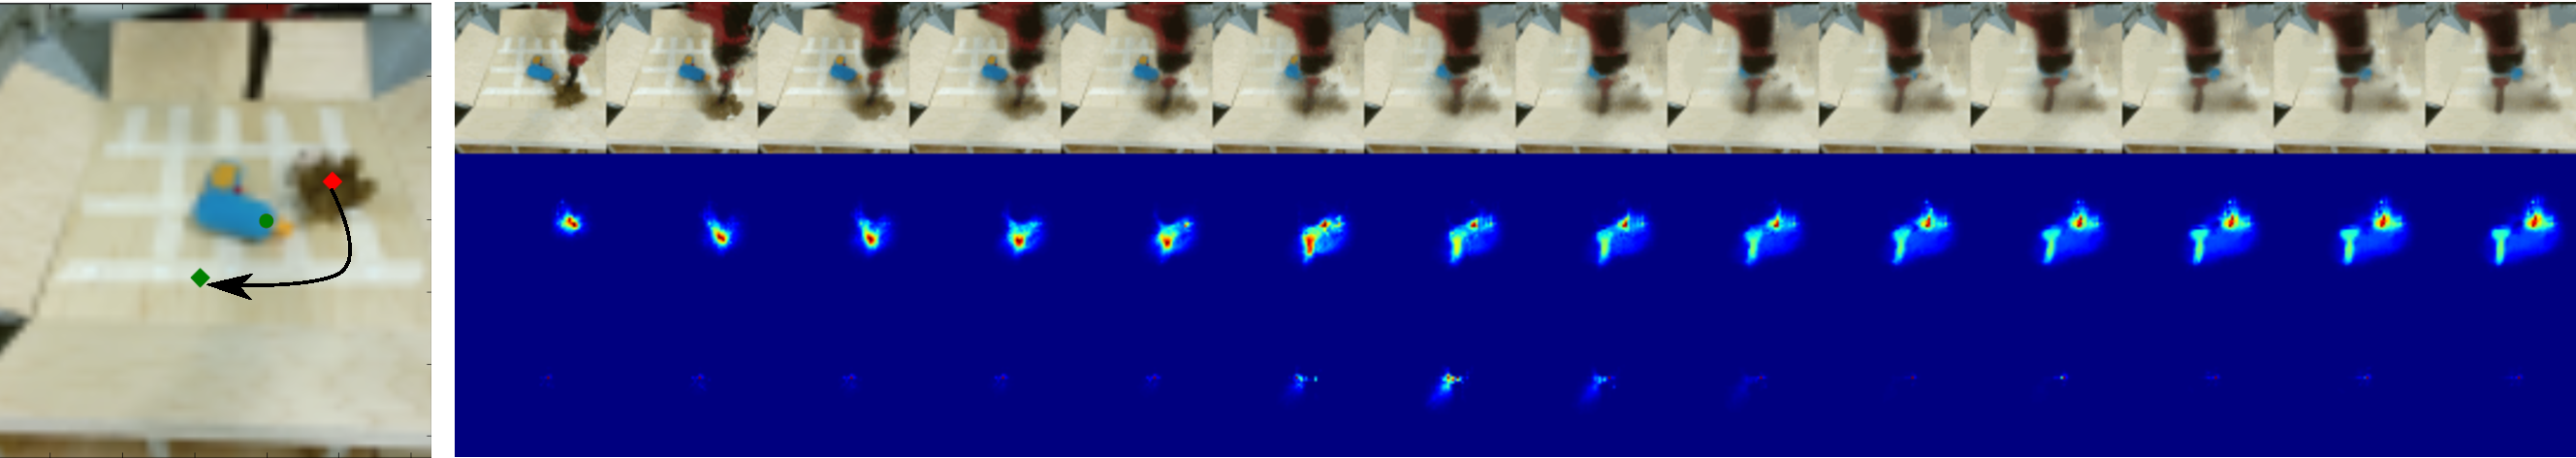
\includegraphics[width=1\linewidth]{images_sna/multiobject_qualitative/avoid_obstacle.pdf}
	\caption{Left: Task setup with green dot marking the obstacle. Right, first row: the predicted frames generated by SNA. Second row: the probability distribution of the designated pixel on the \textit{moving} object (brown stuffed animal). Note that part of the distribution shifts down and left, which is the indicated goal. Third row: the probability distribution of the designated pixel on the obstacle-object (blue power drill). Although the distribution increases in entropy during the occlusion (in the middle), it then recovers and remains on its original position.
		\label{fig:goingaroundocclusion}}
\end{figure*}


\section{Simulated Experiments}
%\todo{shorten if necessary}

In order to provide a more controlled comparison, we also set up a realistic simulation environment using MuJoCo \cite{todorov2012mujoco}, which includes a robotic manipulator controlled via Cartesian position control, similar to our real world setup, pushing randomly-generated L-shaped objects with random colors (see details in supplementary materials). 
We trained the same video prediction model in this environment, and set up 50 evaluation tasks where blocks must be pushed to target locations with maximum episode lengths of 120 steps. 
We  compare our proposed registration-based method, ``predictor propagation,'' and ground-truth registration obtained from the simulator, which provides an oracle upper bound on registration performance. 

%\autoref{fig:sim_bench} shows the results of this simulated evaluation, where the x-axis shows different distance thresholds, and the y-axis shows the fraction of evaluation scenarios where each method pushed the object within that threshold. We can see that, for thresholds around 0.1, our method drastically outperforms predictor propagation (i.e., prior work~\cite{sna}), and has a relatively modest gap in performance against ground-truth tracking. This indicates that our registration method is highly effective in guiding visual MPC, despite being entirely self-supervised.









% that's all folks
\end{document}


